\documentclass[11pt,a4paper]{article}
\usepackage{fontspec,amsmath,amssymb,graphicx,booktabs,longtable,tabularx,array,geometry,caption,hyperref,needspace,pdflscape}
\IfFontExistsTF{Times New Roman}{\setmainfont{Times New Roman}}{\setmainfont{Latin Modern Roman}}
\geometry{left=20mm,right=20mm,top=18mm,bottom=19mm}
\hypersetup{colorlinks=true,urlcolor=blue,linkcolor=black,pdftitle={HiCARE: facility profiles and stratified calibration}}
\urlstyle{same}
\setlength{\parindent}{0pt}
\setlength{\parskip}{5pt plus 1pt}
\setlength{\emergencystretch}{2em}
\setlength{\abovedisplayskip}{7pt}
\setlength{\belowdisplayskip}{7pt}
\captionsetup{font=small,labelfont=bf,justification=raggedright,singlelinecheck=false}
\newcommand{\mainheading}[1]{\par\needspace{4\baselineskip}\vspace{7pt}{\large\bfseries #1}\par\vspace{3pt}}
\newcommand{\subheading}[1]{\par\needspace{3\baselineskip}\vspace{5pt}{\bfseries #1}\par\vspace{1pt}}
\newcolumntype{L}[1]{>{\raggedright\arraybackslash}p{#1}}
\begin{document}
\fontsize{10.5}{13}\selectfont
\renewcommand{\thefigure}{S\arabic{figure}}\renewcommand{\thetable}{S\arabic{table}}\renewcommand{\theequation}{S\arabic{equation}}{\raggedright\LARGE\bfseries Supplementary Appendix\par}\vspace{5pt}
{\large Detailed methods, complete numerical results and extended interpretation\par}\vspace{10pt}
\mainheading{Guide to the Supplementary Appendix}
This appendix accompanies the main manuscript, which retains 27 figures. Supplementary figures are numbered S1–S6 and all 14 tables are numbered S1–S14. Reference numbers follow the main text. Section S1 provides detailed methods and evaluation conditions, S2 contains numerical results, S3 presents supplementary figures and S4 extends the interpretation of the main-text figures. Original result plots retain their data and vector content; main-text Figures 1 and 3 summarise the analytical framework and detailed modelling protocols. Legacy labels “reference LR” and “reference model” denote LR-7, and “CARE v1” denotes EW. In geographic evaluation, the HiCARE label denotes the profile ensemble configuration.

\mainheading{S1 Detailed methods and evaluation conditions}
\subheading{S1.1 Study cohort and unit of analysis}
Data came from Ecuador’s National Institute of Statistics and Censuses (INEC) hospital-bed and discharge registry and historical annual releases [33]. ARI admissions in 2015–2023 were selected using principal ICD-10 diagnoses J00–J06, J09–J18, J20–J22, J85–J86 and U07.1–U07.2. We excluded 632 records admitted before 2015 and 14 records coded as COVID-19 but admitted before 2020. The outcome was in-hospital death recorded at discharge. Children were defined as ages 0–19 and adults as ages 20 or older. The final cohort comprised 576,195 admissions, including 295,225 paediatric admissions with 1,575 deaths and 280,970 adult admissions with 39,473 deaths. A further 9,463,108 non-ARI discharge records informed facility profiles. The case definition excluded perinatal respiratory conditions, which also limits the scope of infant analyses [19].

The admission was the unit of analysis. Public records lacked identifiers linking admissions to individual patients and directly usable hospital identifiers. We therefore defined a facility group by the combination of hospital canton, facility class, administering entity and urban or rural location; a group could include multiple hospitals. Principal diagnoses came from discharge records, supporting retrospective risk monitoring. Individual length of stay, discharge date and outcome-derived fields were excluded from the main individual predictors. Missing categories were represented separately, and unseen categories were treated as missing.

\subheading{S1.2 Probability references for distinct monitoring questions}
Two types of probability served different monitoring purposes. For admission i, let $y_i$ denote the outcome, $x_i$ the coded patient characteristics, $h_i$ the facility group and $t_i$ the admission month. HiCARE estimated mortality risk $p_i$ using patient, facility and historical context. An independent standardisation model estimated reference risk $q_i$ from a restricted predictor set. Summing $q_i$ within group g gave expected deaths $E_g$, which were compared with observed deaths $O_g$ to form the standardised mortality ratio $\mathrm{SMR}_g$.

\begin{equation}
O_g=\sum_{i\in g}y_i,\quad E_g=\sum_{i\in g}q_i,\quad \mathrm{SMR}_g=O_g/E_g.
\end{equation}
The information sets differed because prediction and comparison treat facility differences differently. Prediction uses facility information to identify risk, whereas regional comparison retains outcome differences after adjusting patient case mix. Provincial and facility reference probabilities $q_i$ were therefore estimated with a separate LightGBM model largely restricted to clinical codes and calendar variables. Comparisons of non-COVID outcomes across periods additionally fixed the pre-pandemic model, ensuring a common historical risk relationship.

\subheading{S1.3 Historical context and non-ARI facility profiles}
Patient predictors included age and its recorded unit, sex, ethnicity, residence, diagnostic codes and infection type, admission calendar, facility attributes, and indicators of cross-province or cross-canton care. Recent epidemic context comprised ARI admissions, the COVID-19 share and mortality over the preceding three months, calculated nationally and for selected geographic levels. Recent facility ARI volume relative to the previous year described changes in admission scale. These variables were calendar-lagged. Historical deaths were grouped by admission month; information limitations arising from reporting delays are discussed in Section 6.4.

Recent ARI context described epidemic conditions, whereas historical non-ARI records described more persistent service characteristics. For each facility group and target month, non-ARI records discharged during the preceding 12 months generated 18 profile variables. Seven service statistics comprised discharge volume, all-cause in-hospital mortality, deaths within 48 hours as a proportion of all deaths, mean length of stay capped at 60 days, the proportions aged 0–19 and at least 65, and the proportion receiving cross-canton care. Eleven diagnostic-chapter proportions completed the profile. Proportions were set to missing with fewer than 30 historical records; the early-death proportion additionally required at least ten deaths. Profiles in province-held-out evaluation used the same rules applied to local historical non-ARI data.

\subheading{S1.4 Stratified calibration and nested fitting}
Base learners were LightGBM [34] and XGBoost [35]. LightGBM used a learning rate of 0.05, 127 leaves, a minimum of 80 records per leaf and an L2 penalty of 5. XGBoost used a learning rate of 0.05, maximum depth 8, minimum child weight 5 and an L2 penalty of 5. Both used feature and row subsampling fractions of 0.8, up to 4,000 rounds, and early stopping on a stratified 10\% training holdout with patience of 100 rounds. The equal-weight comparator additionally included TabM [4]. Member probabilities were averaged and then logistically recalibrated using internal held-out predictions.

Equal weighting applies the same model combination to all patients, although children and COVID-19 patients occupy different risk ranges. To allow their combinations to differ, member probabilities were clipped to [$10^{-7}$, 1$-$$10^{-7}$], transformed to logits $z_i^{(m)}$, and combined through logistic stacking with regularisation parameter C = 1000. The child indicator $c_i$ and COVID-19 indicator $v_i$ interacted with member scores to produce the stratified score in equation (S2).

\begin{equation}
z_i^A=\alpha+\sum_m a_mz_i^{(m)}+c_i\left(b+\sum_m b_mz_i^{(m)}\right)+v_i\left(d+\sum_m d_mz_i^{(m)}\right).
\end{equation}
These interactions addressed prespecified age and infection strata, but systematic errors could remain across other registry variables within each stratum. Starting from stacking score $z_i^A$, a shallow residual function h was fitted using variables $u_i$ comprising age, sex, ethnicity, urban or rural residence, sector, infection type, administering entity, facility class, province and month. This yielded the corrected score in equation (S3).

\begin{equation}
z_i^B=z_i^A+h(u_i,z_i^A).
\end{equation}
The residual learner used 8 leaves, at least 1,000 records per leaf, a learning rate of 0.03, an L2 penalty of 20, and feature and row subsampling fractions of 0.8, with at most 500 rounds. Fifteen per cent of nested training records provided early stopping with patience of 30 rounds. In-distribution analyses included year; temporal extrapolation did not use unseen year categories.

Residual learning primarily optimised record-level log loss. Because subsequent monitoring also aggregates expected deaths, an unpenalised logistic projection was fitted to the corrected score and specified marginal categories. Indicators $g_k$ covered age group, sex, ethnicity, urban or rural residence, sector and infection type, with year added in the in-distribution configuration. Equation (S4) gives the resulting probability.

\begin{equation}
p_i^H=\sigma\!\left(\beta_0+\beta_1z_i^B+\sum_k\gamma_kg_k(i)\right),\quad\sigma(s)=(1+e^{-s})^{-1}.
\end{equation}
When a finite maximum-likelihood solution exists and optimisation converges sufficiently, the category score equations imply approximately zero sums of $g_k(i)$($y_i$$-$$p_i^H$). Predicted deaths therefore approach observed deaths in the corresponding marginal categories of the fitting sample. This provides an explicit aggregation target, whose held-out performance was evaluated on independent outer-fold records. Projection used all nested training rows and shared some outcomes with residual learning. The 15\% holdout served only residual early stopping, not independent projection calibration.

In-distribution evaluation used five stratified outer folds. For each outer test fold, one of the other four folds was held out in turn while the remaining three trained the base model, yielding nested predictions. The second layer was fitted on these predictions and applied to the outer test records. Each base learner therefore involved 20 outer–inner combinations. Historical context was precomputed by calendar before splitting, so national historical mortality features could contain outcomes from earlier months of held-out records. The protocol evaluates a retrospective setting with historical monitoring information, as discussed in Section 6.4.

\subheading{S1.5 Monthly state updating}
Group calibration established the development-period mapping, and temporal evaluation assessed its adaptation to later months. Base models used 2015–2021 data, the second layer used internal five-fold predictions from that period, and 2022–2023 formed the temporal test set. The vector $\phi_i$ = [1, $z_i^H$, $v_i$, $c_i$]\textasciicircum{}T contained an intercept, the original score, a COVID-19 indicator and a child indicator. Month-specific coefficients $\theta_t$ adjusted the mapping as in equation (S5).

\begin{equation}
\operatorname{logit}(p_{i,t})=\phi_i^\top\theta_t,\quad\theta_t=\theta_{t-1}+\varepsilon_t,\quad\varepsilon_t\sim N(0,qI).
\end{equation}
Each month was predicted using the previous month’s state, followed by a Laplace-approximation update once that month’s outcomes were available. Development used forward validation in 2018–2021 to compare three coefficient configurations and q values of 0.001, 0.01 and 0.1. Log loss selected the four-dimensional state with q = 0.1. Initial covariance was 0.05I, with at most 25 Newton iterations per update and convergence tolerance $10^{-8}$. The simulation followed admission months retrospectively; internal records used for initialisation also contributed to projection fitting.

\subheading{S1.6 Case-mix standardisation}
Regional and facility comparisons used a separate LightGBM with age and its unit, sex, three- and four-character ICD codes, infection type, admission month, national historical epidemic context and year. Residence, ethnicity and facility attributes were excluded. Five-fold out-of-fold probabilities were followed by a common intercept and slope fitted to all out-of-fold predictions and outcomes, aligning overall observed and expected deaths. This step established an indirect standardisation reference and was not an independent assessment of predictive performance.

With few admissions, a small number of deaths can produce large O/E fluctuations. A Gamma–Poisson empirical Bayes model stabilised comparisons across different count scales by shrinking less precise ratios towards the overall level, as specified in equation (S6).

\begin{equation}
O_g\mid\theta_g\sim\operatorname{Poisson}(E_g\theta_g),\quad\theta_g\sim\operatorname{Gamma}(a,a),\quad\theta_g\mid O_g,E_g\sim\operatorname{Gamma}(O_g+a,E_g+a).
\end{equation}
The Gamma distribution used shape–rate parameterisation, with a estimated by marginal likelihood. The posterior mean was ($O_g$+a)/($E_g$+a), and its 2.5th and 97.5th percentiles defined a 95\% shrinkage interval. Provinces and facility groups required at least 300 admissions and five expected deaths; administering-entity and facility-class summaries required at least 500 admissions and five expected deaths. Groups with an interval lower bound above 1 were flagged as above reference. Intervals conditioned on fixed expected counts, did not propagate all uncertainty in model fitting or estimation of a, and were not adjusted for multiple screening comparisons.

\subheading{S1.7 Non-COVID outcomes and demographic disparities}
Non-COVID period comparisons used a clinical LightGBM trained only on 2015–2019 records, retaining age, sex, diagnosis and admission month but excluding year and epidemic context. Pre-pandemic out-of-fold predictions provided overall recalibration, after which the mapping was fixed. O$-$E measured the death difference from this historical case-mix reference; O/E intervals used Poisson count methods. Facility COVID-19 demand was proxied by current monthly COVID-19 admissions relative to the same facility’s pre-pandemic ARI baseline. This measures demand changes without a bed or staffing capacity denominator.

Demographic comparisons successively reported crude mortality rate ratios, relative O/E after clinical case-mix adjustment, and relative O/E after additionally including facility location, class, sector and non-ARI profiles. For target group g and reference group r, the ratio is defined in equation (S7).

\begin{equation}
R_{g:r}=\frac{O_g/E_g}{O_r/E_r}.
\end{equation}
Neither standardisation model directly included ethnicity, urban or rural residence, or cross-canton care indicators. Relative-ratio intervals used 400 record-level bootstrap samples without refitting risk models or clustering by facility or patient. Successive adjustments describe conditional associations, not causal mediation. In particular, adding sector-related predictors in public–private comparisons moves the comparison towards outcomes conditional on sector.

\subheading{S1.8 Paediatric demand and interpretable risk groups}
Monthly counts from 2015–2019 were fitted with a Poisson model containing seasonal terms and a log-population offset to estimate expected admissions and deaths from 2020 onwards. A linear time trend was added for sensitivity analysis. Parameter simulation and count sampling allowing overdispersion generated 2,000 predictive draws. Infant and age 1–4 analyses shared the population trajectory for ages 0–4 because separate series were unavailable, making fine age-specific estimates exploratory.

A shallow tree with 14 leaves was fitted on 80\% of records to describe where risk was concentrated. Mortality, admission shares and death shares for each phenotype were reported in the remaining 20\%. The tree compressed risk patterns, and its data-driven age cut-offs differ from the prespecified paediatric definition of 0–19 years. Mortality-concentration curves compared the proportions of deaths captured when prioritising a given share of records, informing potential future manual review.

\subheading{S1.9 Evaluation tasks and comparator configurations}
Comparators comprised seven-variable logistic regression, LR-7 (age group, sex, ethnicity, urban or rural residence, public or private sector, infection type and year), an equal-weight LightGBM/XGBoost/TabM ensemble, EW, and HiCARE with facility profiles and stratified calibration. Legacy “reference LR” or “reference model” labels denote LR-7; “CARE v1” denotes EW. Component analyses assessed profiles, stratified stacking, residual correction, projection, year and a single-LightGBM configuration. Development, held-out evaluation and intended uses were distinguished following TRIPOD+AI [29].

Evaluation comprised five-fold in-distribution cross-validation, temporal holdout in 2022–2023 and six-fold province-grouped holdout. The latter compared ensembles without geographic identifiers. The no-profile configuration also removed regional and facility epidemic context; the profile configuration added non-ARI profiles. This protocol used equal-weight ensembling and recalibration, not the full HiCARE second layer. The no-profile configuration included LightGBM, XGBoost and TabM, whereas the profile configuration included LightGBM and XGBoost. Differences therefore involved both profiles and ensemble membership. The geographic HiCARE label is interpreted throughout as the geographic profile configuration.

Discrimination used AUROC and AUPRC calculated as average precision; probability errors used Brier score and log loss. Calibration intercepts were estimated with slope fixed at 1 and had ideal value 0; ideal calibration slope was 1. ICI used weighted isotonic approximation over 200 predicted-risk quantile bins, and ECE used risk quantile bins. Subgroup O/E required at least 25 deaths and 25 survivors. Summaries reported sample-size-weighted mean and maximum absolute log(O/E). Worst-group ECE used ten quantile bins and required at least 5,000 records. Marginal groups could overlap, and these metrics do not represent every intersecting population.

Decision curves measured net benefit as TP/N $-$ FP/N $\times$ $\tau$/(1$-$$\tau$) at threshold $\tau$. Concentration curves reported mortality coverage among prioritised records. Both assessed potential priority information without a prespecified clinical intervention or verified availability at admission. Paired bootstrap intervals resampled records, and the main training runs used a single random seed. The “best LR-7” in temporal testing was selected retrospectively from nine variants by test-period log loss, a comparison favourable to the baseline.

\clearpage
\mainheading{S2 Complete numerical results}
\begingroup\fontsize{8}{9.5}\selectfont\setlength{\tabcolsep}{1.1mm}\renewcommand{\arraystretch}{1.2}
\begin{longtable}{@{}L{31.43mm}L{86.01mm}L{47.97mm}@{}}
\caption{Inputs, operations and purposes of HiCARE components.}\label{tab:components}\\
\toprule
Component & Content & Purpose \\
\midrule\endfirsthead
\multicolumn{3}{l}{\small Table S1 continued}\\
\toprule
Component & Content & Purpose \\
\midrule\endhead
\bottomrule\endfoot
Facility service profiles & Previous 12 months of non-ARI discharges: volume, mortality, early-death share, length of stay, age, cross-canton care and 11 diagnostic categories; 9,463,108 historical records & Supplement facility identifiers with comparable service characteristics \\
Base learners & LightGBM and XGBoost; 33 base variables plus 18 facility-profile features in the current feature list; TabM included in EW & Estimate individual mortality risk \\
Stratified stacking (2a) & Member logits with separate combination weights for children and COVID-19 & Accommodate population risk heterogeneity \\
Residual correction (2b) & Shallow boosted trees on subgroup variables, initialised with the stacked logit & Reduce systematic errors associated with specified variables \\
Marginal projection (2c) & Unpenalised logistic fit using corrected score, age, sex, ethnicity, urban/rural residence, sector and infection type; year added in distribution & Constrain average residuals within included marginal categories in the fitting sample \\
Monthly state updating & Update intercept, slope, COVID-19 and child offsets under a random walk & Track probability drift in later periods \\
Nested fitting & Train the second layer on nested predictions; base learners do not directly use corresponding outer test records & Separate direct second-layer fitting from outer testing; historical information requires separate assessment \\
\end{longtable}\endgroup
{\small Marginal residual constraints apply to the projection fitting data and included categories. Historical-information boundaries are described in the main text.\par}
HiCARE components address distinct sources of risk information and probability error (Table S1). Facility profiles first extend the information available to base models. Stratified stacking then allows different score combinations for children and COVID-19 patients. Residual correction learns remaining errors associated with specified group variables, and marginal projection constrains fitted group-level totals. Monthly updating subsequently addresses shifts in later periods. Tables S4 and S5 assess within-period component gains and temporal maintenance, respectively.


\clearpage
\begingroup\fontsize{8}{9.5}\selectfont\setlength{\tabcolsep}{1.1mm}\renewcommand{\arraystretch}{1.2}
\begin{longtable}{@{}L{50.11mm}L{17.75mm}L{17.75mm}L{17.75mm}L{17.75mm}L{17.75mm}L{17.75mm}@{}}
\caption{Development configurations for monthly state updating, evaluated by forward validation in 2018–2021 and selected by development-period log loss.}\label{tab:dyn}\\
\toprule
Updated coefficients & Drift variance & Log loss & Brier & Calibration intercept & Slope & ICI \\
\midrule\endfirsthead
\multicolumn{7}{l}{\small Table S2 continued}\\
\toprule
Updated coefficients & Drift variance & Log loss & Brier & Calibration intercept & Slope & ICI \\
\midrule\endhead
\bottomrule\endfoot
Intercept & 0.001 & 0.2592 & 0.0794 & +0.042 & 0.906 & 0.0098 \\
Intercept & 0.01 & 0.2583 & 0.0792 & +0.031 & 0.911 & 0.0092 \\
Intercept & 0.1 & 0.2580 & 0.0791 & +0.026 & 0.913 & 0.0090 \\
Intercept + slope & 0.001 & 0.2585 & 0.0792 & +0.028 & 0.969 & 0.0059 \\
Intercept + slope & 0.01 & 0.2581 & 0.0791 & +0.022 & 0.969 & 0.0063 \\
Intercept + slope & 0.1 & 0.2580 & 0.0791 & +0.019 & 0.966 & 0.0064 \\
Intercept + slope + COVID-19 and child offsets & 0.001 & 0.2567 & 0.0788 & -0.003 & 0.969 & 0.0053 \\
Intercept + slope + COVID-19 and child offsets & 0.01 & 0.2563 & 0.0787 & -0.005 & 0.975 & 0.0049 \\
Intercept + slope + COVID-19 and child offsets & 0.1 & 0.2561 & 0.0786 & -0.008 & 0.974 & 0.0048 \\
One-month rolling window (EW) & — & 0.2578 & 0.0791 & +0.023 & 0.916 & 0.0089 \\
\end{longtable}\endgroup
{\small Configuration selection used 2018–2021 forward validation. The rolling-window row is a development comparator, not an additional test result.\par}
The four-dimensional state with q = 0.1 achieved the lowest development log loss of 0.2561 and an ICI of 0.0048 (Table S2). Compared with updating a common intercept alone, adding the score slope and group offsets accommodated changes in both the risk scale and between-group relationships. This configuration was fixed for subsequent temporal testing and compared with static models and rolling windows to assess whether the development-period choice remained effective in 2022–2023.


\clearpage
\begingroup\fontsize{8}{9.5}\selectfont\setlength{\tabcolsep}{1.1mm}\renewcommand{\arraystretch}{1.2}
\begin{longtable}{@{}L{13.70mm}L{38.05mm}L{14.35mm}L{14.35mm}L{14.35mm}L{14.35mm}L{14.35mm}L{14.35mm}L{14.35mm}@{}}
\caption{Performance of LR-7, EW and HiCARE under three evaluation protocols (random seed 0).}\label{tab:perf}\\
\toprule
Population & Model & AUROC & AUPRC & Brier & Log loss & ICI & Calibration intercept & Slope \\
\midrule\endfirsthead
\multicolumn{9}{l}{\small Table S3 continued}\\
\toprule
Population & Model & AUROC & AUPRC & Brier & Log loss & ICI & Calibration intercept & Slope \\
\midrule\endhead
\bottomrule\endfoot
\multicolumn{9}{p{167mm}}{\bfseries Five-fold cross-validation}\\
All ages & LR-7 & 0.859 & 0.296 & 0.0563 & 0.1934 & 0.0057 & -0.000 & 0.999 \\
All ages & EW (equal weight) & 0.903 & 0.416 & 0.0508 & 0.1707 & 0.0021 & 0.013 & 0.993 \\
All ages & HiCARE & 0.904 & 0.419 & 0.0507 & 0.1701 & 0.0016 & -0.005 & 1.003 \\
Children & LR-7 & 0.689 & 0.015 & 0.0053 & 0.0318 & 0.0006 & 0.001 & 0.881 \\
Children & EW (equal weight) & 0.874 & 0.076 & 0.0051 & 0.0266 & 0.0009 & 0.081 & 1.067 \\
Children & HiCARE & 0.874 & 0.081 & 0.0051 & 0.0265 & 0.0006 & -0.009 & 0.984 \\
Adults & LR-7 & 0.729 & 0.303 & 0.1099 & 0.3633 & 0.0117 & -0.000 & 1.006 \\
Adults & EW (equal weight) & 0.815 & 0.426 & 0.0988 & 0.3221 & 0.0036 & 0.010 & 0.991 \\
Adults & HiCARE & 0.817 & 0.429 & 0.0985 & 0.3210 & 0.0033 & -0.005 & 1.006 \\
\multicolumn{9}{p{167mm}}{\bfseries Temporal test 2022–2023 (update configurations in model labels and note)}\\
All ages & LR-7 (best of nine variants) & 0.868 & 0.195 & 0.0336 & 0.1252 & 0.0034 & -0.045 & 0.975 \\
All ages & EW + rolling window & 0.898 & 0.262 & 0.0326 & 0.1177 & 0.0079 & -0.108 & 0.860 \\
All ages & HiCARE & 0.900 & 0.266 & 0.0323 & 0.1163 & 0.0052 & -0.097 & 0.924 \\
Children & LR-7 (best of nine variants) & 0.665 & 0.009 & 0.0041 & 0.0261 & 0.0007 & -0.099 & 0.842 \\
Children & EW + rolling window & 0.841 & 0.044 & 0.0040 & 0.0228 & 0.0008 & 0.112 & 1.036 \\
Children & HiCARE & 0.843 & 0.045 & 0.0041 & 0.0227 & 0.0011 & -0.112 & 1.006 \\
Adults & LR-7 (best of nine variants) & 0.693 & 0.204 & 0.0876 & 0.3066 & 0.0084 & -0.040 & 0.915 \\
Adults & EW + rolling window & 0.757 & 0.274 & 0.0848 & 0.2916 & 0.0204 & -0.126 & 0.779 \\
Adults & HiCARE & 0.764 & 0.279 & 0.0839 & 0.2879 & 0.0138 & -0.096 & 0.852 \\
\multicolumn{9}{p{167mm}}{\bfseries Unseen provinces (without location identifiers)}\\
All ages & LR-7 & 0.848 & 0.269 & 0.0574 & 0.1982 & 0.0082 & -0.039 & 0.912 \\
All ages & EW (no location) & 0.865 & 0.319 & 0.0560 & 0.1913 & 0.0100 & -0.004 & 0.856 \\
All ages & HiCARE (no location + profiles) & 0.875 & 0.321 & 0.0554 & 0.1876 & 0.0101 & 0.171 & 0.921 \\
Children & LR-7 & 0.670 & 0.014 & 0.0053 & 0.0321 & 0.0010 & -0.003 & 0.760 \\
Children & EW (no location) & 0.813 & 0.036 & 0.0052 & 0.0292 & 0.0007 & 0.049 & 0.909 \\
Children & HiCARE (no location + profiles) & 0.825 & 0.042 & 0.0052 & 0.0286 & 0.0006 & 0.067 & 0.984 \\
Adults & LR-7 & 0.706 & 0.275 & 0.1122 & 0.3726 & 0.0165 & -0.041 & 0.845 \\
Adults & EW (no location) & 0.737 & 0.327 & 0.1093 & 0.3617 & 0.0201 & -0.007 & 0.785 \\
Adults & HiCARE (no location + profiles) & 0.757 & 0.328 & 0.1082 & 0.3547 & 0.0203 & 0.176 & 0.857 \\
\end{longtable}\endgroup
{\small Geographic HiCARE denotes the profile ensemble configuration. Temporal EW uses a rolling window; matched state-updating comparisons are reported in Table S5.\par}
In all-age cross-validation, HiCARE achieved an AUROC of 0.904 compared with 0.859 for LR-7, and log loss decreased from 0.1934 to 0.1701 (Table S3). Age-specific results showed that this improvement was not solely due to the large mortality difference between children and adults. Paediatric AUROC increased from 0.689 to 0.874 and AUPRC from 0.015 to 0.081; adult AUROC increased from 0.729 to 0.817. Expanded information and nonlinear modelling therefore improved risk identification within age strata, supporting review among comparable patients.

The advantage was much smaller against EW, whose all-age AUROC was already 0.903. The base ensemble had extracted most ranking information. HiCARE reduced ICI from 0.0021 to 0.0016, locating its incremental value more specifically in probability accuracy. Risk curves and group errors clarify the source of that increment.


\clearpage
\begin{landscape}
\begingroup\fontsize{8}{9.5}\selectfont\setlength{\tabcolsep}{1.1mm}\renewcommand{\arraystretch}{1.2}
\begin{longtable}{@{}L{72.00mm}L{18.67mm}L{18.67mm}L{18.67mm}L{18.67mm}L{18.67mm}L{18.67mm}L{18.67mm}L{18.67mm}L{18.67mm}@{}}
\caption{Cross-validation results for facility profiles and calibration components. The final three columns summarise calibration in specified subgroups.}\label{tab:layers}\\
\toprule
Model & AUROC & Log loss & ICI & Calibration intercept & Child calibration intercept & Child AUPRC & Mean |log(O/E)| & Max |log(O/E)| & Worst ECE \\
\midrule\endfirsthead
\multicolumn{10}{l}{\small Table S4 continued}\\
\toprule
Model & AUROC & Log loss & ICI & Calibration intercept & Child calibration intercept & Child AUPRC & Mean |log(O/E)| & Max |log(O/E)| & Worst ECE \\
\midrule\endhead
\bottomrule\endfoot
LR-7 & 0.8591 & 0.1934 & 0.0057 & -0.0001 & +0.001 & 0.015 & 0.0006 & 0.022 & 0.0183 \\
EW: equal weighting + held-out recalibration & 0.9028 & 0.1707 & 0.0021 & +0.0135 & +0.081 & 0.076 & 0.0219 & 0.201 & 0.0076 \\
LightGBM + facility profiles & 0.9034 & 0.1704 & 0.0026 & +0.0095 & -0.005 & 0.083 & 0.0132 & 0.142 & 0.0075 \\
Equal weighting + facility profiles & 0.9033 & 0.1704 & 0.0017 & +0.0135 & +0.094 & 0.079 & 0.0229 & 0.220 & 0.0068 \\
+ Stratified stacking (2a) & 0.9035 & 0.1703 & 0.0017 & -0.0052 & +0.019 & 0.080 & 0.0126 & 0.178 & 0.0064 \\
+ Residual correction (2b) & 0.9037 & 0.1701 & 0.0017 & -0.0038 & +0.019 & 0.080 & 0.0089 & 0.166 & 0.0050 \\
+ Marginal projection (2c) = HiCARE & 0.9037 & 0.1701 & 0.0016 & -0.0052 & -0.009 & 0.081 & 0.0054 & 0.076 & 0.0059 \\
HiCARE without period terms & 0.9036 & 0.1702 & 0.0014 & -0.0049 & -0.008 & 0.080 & 0.0088 & 0.079 & 0.0068 \\
HiCARE with LightGBM only & 0.9037 & 0.1701 & 0.0015 & -0.0045 & -0.009 & 0.084 & 0.0048 & 0.067 & 0.0059 \\
\end{longtable}\endgroup
{\small Mean and maximum errors use 42 specified marginal groups. Worst-group ECE uses ten within-group risk quantile bins among groups meeting the sample-size criterion.\par}
After adding profiles, the equal-weight configuration achieved an AUROC of 0.9033, but mean subgroup absolute log(O/E) remained 0.0229 (Table S4). Adding useful risk information and correcting predicted group totals were therefore distinct steps. Stratified stacking, residual correction and marginal projection successively reduced mean error to 0.0126, 0.0089 and 0.0054 while AUROC stayed between 0.9035 and 0.9037. These steps primarily changed probability allocation within a similar ranking, bringing expected deaths closer to observed counts.

Relative to the original EW, final mean error decreased by approximately 75.3\%, maximum absolute log(O/E) decreased from 0.201 to 0.076, and AUROC increased by only 0.0009. Gains in probability aggregation exceeded gains in ranking. A single-LightGBM configuration achieved an AUROC of 0.9037 and log loss of 0.1701, retaining these gains with a simpler learner. Ensemble complexity was therefore not the principal determinant of performance in this comparison.


\end{landscape}
\clearpage
\begingroup\fontsize{8}{9.5}\selectfont\setlength{\tabcolsep}{1.1mm}\renewcommand{\arraystretch}{1.2}
\begin{longtable}{@{}L{51.75mm}L{12.56mm}L{12.56mm}L{12.56mm}L{12.56mm}L{12.56mm}L{12.56mm}L{12.56mm}L{12.56mm}@{}}
\caption{Static, rolling-window and state-space updating configurations in all-age temporal testing in 2022–2023.}\label{tab:temporal}\\
\toprule
Model (trained in 2015–2021) & AUROC & AUPRC & Brier & Log loss & ICI & Calibration intercept & Slope & O/E \\
\midrule\endfirsthead
\multicolumn{9}{l}{\small Table S5 continued}\\
\toprule
Model (trained in 2015–2021) & AUROC & AUPRC & Brier & Log loss & ICI & Calibration intercept & Slope & O/E \\
\midrule\endhead
\bottomrule\endfoot
LR-7, unseen year mapped to 2015 & 0.865 & 0.178 & 0.0340 & 0.1267 & 0.0062 & -0.13 & 0.99 & 0.90 \\
LR-7, latest year carried forward & 0.865 & 0.178 & 0.0360 & 0.1337 & 0.0259 & -0.61 & 0.99 & 0.60 \\
LR-7, no year & 0.862 & 0.175 & 0.0351 & 0.1302 & 0.0143 & -0.35 & 0.88 & 0.75 \\
Unseen year as 2015 + rolling window & 0.866 & 0.186 & 0.0338 & 0.1263 & 0.0050 & 0.04 & 0.97 & 1.04 \\
Latest year + rolling window & 0.867 & 0.192 & 0.0337 & 0.1260 & 0.0054 & -0.05 & 0.94 & 0.96 \\
No year + rolling window & 0.862 & 0.183 & 0.0342 & 0.1281 & 0.0088 & -0.06 & 0.86 & 0.95 \\
Unseen year as 2015 + state space & 0.867 & 0.190 & 0.0337 & 0.1256 & 0.0034 & 0.06 & 1.02 & 1.05 \\
Latest year + state space & 0.868 & 0.195 & 0.0336 & 0.1252 & 0.0034 & -0.05 & 0.98 & 0.96 \\
No year + state space & 0.867 & 0.193 & 0.0336 & 0.1254 & 0.0032 & -0.04 & 0.98 & 0.96 \\
EW, static & 0.898 & 0.254 & 0.0341 & 0.1216 & 0.0182 & -0.50 & 0.90 & 0.68 \\
EW + rolling window & 0.898 & 0.262 & 0.0326 & 0.1177 & 0.0079 & -0.11 & 0.86 & 0.92 \\
EW + state space & 0.900 & 0.268 & 0.0322 & 0.1163 & 0.0051 & -0.09 & 0.94 & 0.93 \\
HiCARE, static & 0.899 & 0.247 & 0.0343 & 0.1220 & 0.0196 & -0.53 & 0.91 & 0.66 \\
HiCARE + rolling window & 0.899 & 0.264 & 0.0324 & 0.1169 & 0.0067 & -0.08 & 0.87 & 0.94 \\
HiCARE + state space & 0.900 & 0.266 & 0.0323 & 0.1163 & 0.0052 & -0.10 & 0.92 & 0.93 \\
\end{longtable}\endgroup
Static HiCARE had an O/E of 0.66 in 2022–2023, indicating that the development-period mapping overpredicted later deaths (Table S5). A rolling window increased this ratio to 0.94 and monthly state updating to 0.93. State updating reduced ICI from 0.0196 to 0.0052 and log loss from 0.1220 to 0.1163, while AUROC changed only from 0.899 to 0.900. Maintenance principally adjusted the probabilities associated with existing scores rather than rebuilding their ranking.

Applying the same state update to EW yielded the same log loss of 0.1163 and an ICI of 0.0051. Both models therefore identified changing probability scales as the main temporal problem. Periodic maintenance preserved discrimination while reducing systematic overprediction. LR-7 was closer to ideal on some calibration measures but had lower AUROC, again distinguishing probability scale from risk identification.


\clearpage
\begingroup\fontsize{8}{9.5}\selectfont\setlength{\tabcolsep}{1.1mm}\renewcommand{\arraystretch}{1.2}
\begin{longtable}{@{}L{28.98mm}L{19.32mm}L{19.32mm}L{19.32mm}L{74.06mm}@{}}
\caption{Comparison with LR-7 across 13 metrics. Temporal evaluation uses the best of nine LR-7 variants selected by test log loss.}\label{tab:win}\\
\toprule
Protocol & Population & EW wins & HiCARE wins & Metrics favouring LR-7 over HiCARE \\
\midrule\endfirsthead
\multicolumn{5}{l}{\small Table S6 continued}\\
\toprule
Protocol & Population & EW wins & HiCARE wins & Metrics favouring LR-7 over HiCARE \\
\midrule\endhead
\bottomrule\endfoot
Cross-validation & All ages & 11/13 & 11/13 & Calibration intercept, slope \\
Cross-validation & Children & 10/13 & 11/13 & Calibration intercept, ICI \\
Cross-validation & Adults & 11/13 & 12/13 & Calibration intercept \\
Temporal test 2022–2023 & All ages & 9/13 & 9/13 & Calibration intercept, slope, ECE, ICI \\
Temporal test 2022–2023 & Children & 11/13 & 11/13 & Calibration intercept, ICI \\
Temporal test 2022–2023 & Adults & 9/13 & 9/13 & Calibration intercept, slope, ECE, ICI \\
Unseen provinces & All ages & 10/13 & 10/13 & Calibration intercept, ECE, ICI \\
Unseen provinces & Children & 12/13 & 12/13 & Calibration intercept \\
Unseen provinces & Adults & 10/13 & 10/13 & Calibration intercept, ECE, ICI \\
Total &  & 93/117 & 95/117 &  \\
\end{longtable}\endgroup
{\small Temporal LR-7 was selected by test-period log loss. Protocol-specific HiCARE configurations are defined in Section S1.9.\par}
Across populations and protocols, HiCARE or the corresponding profile configuration outperformed LR-7 in 95 of 117 comparisons, comprising 81 of 81 non-calibration comparisons and 14 of 36 calibration comparisons (Table S6). This contrast agrees with the individual analyses. Expanded models improved discrimination and related performance more consistently, whereas absolute probability accuracy depended more strongly on population and evaluation setting. In-distribution group correction, later-month updating and local recalibration therefore address different needs. The 117 comparisons share records and metric information and describe a performance pattern rather than 117 independent pieces of evidence.


\clearpage
\begin{landscape}
\begingroup\fontsize{8}{9.5}\selectfont\setlength{\tabcolsep}{1.1mm}\renewcommand{\arraystretch}{1.0}
\begin{longtable}{@{}L{32.98mm}L{17.67mm}L{12.96mm}L{15.31mm}L{14.14mm}L{35.34mm}L{24.74mm}L{16.49mm}L{16.49mm}L{16.49mm}L{16.49mm}L{16.49mm}@{}}
\caption{Case-mix-standardised in-hospital mortality ratios by hospital province, with empirical Bayes shrinkage. Expected deaths come from the clinical case-mix model. The final five columns show shrunk ratios by period and age stratum.}\label{tab:prov}\\
\toprule
Province & Admissions & Deaths & Expected & Crude ratio & Standardised (95\% credible interval) & Flag & 2015—19 & 2020—21 & 2022—23 & Children & Adults \\
\midrule\endfirsthead
\multicolumn{12}{l}{\small Table S7 continued}\\
\toprule
Province & Admissions & Deaths & Expected & Crude ratio & Standardised (95\% credible interval) & Flag & 2015—19 & 2020—21 & 2022—23 & Children & Adults \\
\midrule\endhead
\bottomrule\endfoot
El Oro & 27,710 & 3,530 & 2,254 & 1.79 & 1.56 [1.51—1.61] & Above expected & 1.20 & 1.68 & 1.51 & 0.85 & 1.59 \\
Sucumbíos & 6,280 & 474 & 318 & 1.06 & 1.47 [1.34—1.60] & Above expected & 1.21 & 1.50 & 1.56 & 1.43 & 1.46 \\
Manabí & 37,113 & 3,059 & 2,354 & 1.16 & 1.30 [1.25—1.34] & Above expected & 1.01 & 1.35 & 1.51 & 1.49 & 1.29 \\
Esmeraldas & 10,122 & 726 & 573 & 1.01 & 1.26 [1.17—1.35] & Above expected & 0.89 & 1.49 & 1.01 & 1.20 & 1.26 \\
Santo Domingo de los Tsáchilas & 15,862 & 1,542 & 1,257 & 1.36 & 1.22 [1.16—1.29] & Above expected & 0.75 & 1.30 & 1.54 & 0.84 & 1.24 \\
Tungurahua & 26,946 & 2,464 & 2,173 & 1.28 & 1.13 [1.09—1.18] & Above expected & 1.14 & 1.19 & 0.75 & 0.53 & 1.16 \\
Napo & 3,554 & 215 & 192 & 0.85 & 1.11 [0.97—1.26] & Compatible with expected & 0.71 & 1.30 & 1.00 & 0.84 & 1.14 \\
Guayas & 106,639 & 7,723 & 6,953 & 1.02 & 1.11 [1.09—1.14] & Above expected & 1.70 & 0.90 & 1.33 & 1.15 & 1.11 \\
Santa Elena & 8,408 & 521 & 472 & 0.87 & 1.10 [1.01—1.19] & Above expected & 1.07 & 1.09 & 1.20 & 0.30 & 1.14 \\
Carchi & 6,078 & 512 & 465 & 1.18 & 1.10 [1.01—1.19] & Above expected & 0.85 & 1.26 & 0.88 & 0.65 & 1.12 \\
Azuay & 40,903 & 3,431 & 3,231 & 1.18 & 1.06 [1.03—1.10] & Above expected & 1.03 & 1.09 & 1.03 & 1.48 & 1.05 \\
Pastaza & 4,165 & 198 & 191 & 0.67 & 1.03 [0.90—1.18] & Compatible with expected & 0.89 & 1.12 & 0.88 & 0.68 & 1.08 \\
Chimborazo & 21,488 & 1,535 & 1,572 & 1.00 & 0.98 [0.93—1.03] & Compatible with expected & 0.71 & 1.14 & 0.80 & 0.41 & 1.00 \\
Galápagos & 729 & 40 & 43 & 0.77 & 0.96 [0.72—1.22] & Compatible with expected & 0.74 & 1.08 & 0.97 & — & 0.98 \\
Cañar & 12,809 & 755 & 845 & 0.83 & 0.90 [0.83—0.96] & Below expected & 0.75 & 1.10 & 0.60 & 0.41 & 0.92 \\
Orellana & 3,104 & 151 & 176 & 0.68 & 0.87 [0.74—1.01] & Compatible with expected & 0.70 & 0.98 & 0.72 & 0.71 & 0.89 \\
Zamora Chinchipe & 4,260 & 203 & 236 & 0.67 & 0.87 [0.76—0.99] & Below expected & 0.67 & 0.98 & 0.91 & 0.43 & 0.91 \\
Loja & 20,664 & 1,507 & 1,828 & 1.02 & 0.83 [0.79—0.87] & Below expected & 0.58 & 0.97 & 0.75 & 0.43 & 0.84 \\
Imbabura & 17,464 & 1,083 & 1,318 & 0.87 & 0.82 [0.78—0.87] & Below expected & 0.54 & 1.00 & 0.57 & 0.39 & 0.84 \\
Pichincha & 148,923 & 9,166 & 11,409 & 0.86 & 0.80 [0.79—0.82] & Below expected & 0.85 & 0.80 & 0.76 & 0.99 & 0.80 \\
Los Ríos & 19,676 & 1,004 & 1,255 & 0.72 & 0.80 [0.75—0.85] & Below expected & 0.80 & 0.73 & 1.26 & 0.59 & 0.81 \\
Bolívar & 5,663 & 267 & 410 & 0.66 & 0.67 [0.59—0.75] & Below expected & 0.68 & 0.69 & 0.63 & 0.58 & 0.67 \\
Cotopaxi & 13,360 & 605 & 959 & 0.64 & 0.64 [0.59—0.69] & Below expected & 0.67 & 0.60 & 0.77 & 0.74 & 0.63 \\
Morona Santiago & 14,275 & 337 & 565 & 0.33 & 0.61 [0.55—0.67] & Below expected & 0.60 & 0.63 & 0.62 & 0.80 & 0.58 \\
\end{longtable}\endgroup
After case-mix adjustment, shrunk mortality ratios across 24 provinces still ranged from 0.61 to 1.56. The 95\% interval was above 1 in ten provinces and below 1 in nine (Table S7). Age, diagnosis and calendar characteristics explained some variation without making provincial outcomes uniform. Residual differences provide starting points for examining severity, referrals and registry quality.

The same overall ratio could also conceal different temporal and age patterns. High mortality in El Oro was chiefly an adult finding, with a paediatric ratio of 0.85. In Sucumbíos, paediatric and adult ratios were 1.43 and 1.46. Although both provinces had high overall ratios, the populations requiring attention differed. Standardisation thus refined national mortality rankings into geographically and demographically defined review targets.


\end{landscape}
\clearpage
\begingroup\fontsize{8}{9.5}\selectfont\setlength{\tabcolsep}{1.1mm}\renewcommand{\arraystretch}{1.2}
\begin{longtable}{@{}L{24.35mm}L{33.48mm}L{13.48mm}L{13.48mm}L{13.48mm}L{13.48mm}L{13.48mm}L{13.48mm}L{13.48mm}@{}}
\caption{Standardised mortality variation across aggregation levels and adjustment sets. Between-unit standard deviation is the standard deviation of unit effects on the ratio scale under the Gamma prior.}\label{tab:smrsum}\\
\toprule
Unit & Case-mix adjustment & Number of units & Between-unit SD & Above expected & Below expected & 10th–90th percentile & Excess deaths in high-ratio units & Death share \\
\midrule\endfirsthead
\multicolumn{9}{l}{\small Table S8 continued}\\
\toprule
Unit & Case-mix adjustment & Number of units & Between-unit SD & Above expected & Below expected & 10th–90th percentile & Excess deaths in high-ratio units & Death share \\
\midrule\endhead
\bottomrule\endfoot
Province & None (crude) & 24 & 0.32 & 6 & 12 & 0.67—1.25 & 3,523 & 8.6\% \\
Province & Age group, sex, type, year & 24 & 0.25 & 8 & 8 & 0.70—1.33 & 4,257 & 10.4\% \\
Province & Clinical case-mix model & 24 & 0.24 & 10 & 9 & 0.71—1.29 & 3,932 & 9.6\% \\
Administering entity & None (crude) & 11 & 0.57 & 3 & 7 & 0.34—1.19 & 5,283 & 12.9\% \\
Administering entity & Age group, sex, type, year & 11 & 0.43 & 2 & 7 & 0.48—1.09 & 5,192 & 12.6\% \\
Administering entity & Clinical case-mix model & 11 & 0.40 & 1 & 7 & 0.51—1.02 & 4,698 & 11.4\% \\
Facility class & None (crude) & 11 & 0.94 & 5 & 6 & 0.17—2.48 & 7,923 & 19.4\% \\
Facility class & Age group, sex, type, year & 11 & 0.69 & 4 & 5 & 0.62—2.56 & 3,784 & 9.3\% \\
Facility class & Clinical case-mix model & 11 & 0.56 & 4 & 5 & 0.62—2.06 & 3,480 & 8.5\% \\
Facility group & None (crude) & 240 & 1.07 & 51 & 153 & 0.09—1.73 & 12,326 & 30.5\% \\
Facility group & Age group, sex, type, year & 239 & 0.85 & 51 & 141 & 0.18—1.56 & 9,134 & 22.6\% \\
Facility group & Clinical case-mix model & 239 & 0.81 & 49 & 144 & 0.20—1.50 & 8,629 & 21.4\% \\
\end{longtable}\endgroup
Case-mix adjustment reduced between-province standard deviation on the ratio scale from 0.32 to 0.24, approximately one quarter (Table S8). The corresponding facility-group value decreased from 1.07 to 0.81, although included groups changed from 240 to 239. At both levels, patient composition was an important source of outcome variation. Residual variation and changes in high- and low-ratio lists show that standardisation changed both the magnitude of ratios and which units warranted review. Finer facility-level comparisons also require additional severity and referral information.


\clearpage
\begingroup\fontsize{8}{9.5}\selectfont\setlength{\tabcolsep}{1.1mm}\renewcommand{\arraystretch}{1.2}
\begin{longtable}{@{}L{49.23mm}L{21.91mm}L{21.91mm}L{21.91mm}L{21.91mm}L{21.91mm}@{}}
\caption{Standardised mortality ratios by administering entity and facility class.}\label{tab:entity}\\
\toprule
Provider & Admissions & Deaths & Crude ratio & Standardised (95\% credible interval) & Flag \\
\midrule\endfirsthead
\multicolumn{6}{l}{\small Table S9 continued}\\
\toprule
Provider & Admissions & Deaths & Crude ratio & Standardised (95\% credible interval) & Flag \\
\midrule\endhead
\bottomrule\endfoot
\multicolumn{6}{p{167mm}}{\bfseries Administering entity}\\
Ministry of Public Health & 262,062 & 22,145 & 1.19 & 1.27 [1.25—1.29] & Above expected \\
Junta de Beneficencia & 23,274 & 646 & 0.39 & 1.02 [0.95—1.10] & Compatible with expected \\
Ministry of Justice & 951 & 79 & 1.17 & 1.02 [0.81—1.24] & Compatible with expected \\
Other public & 3,794 & 494 & 1.83 & 0.99 [0.91—1.08] & Compatible with expected \\
Social Security (IESS) & 128,563 & 10,742 & 1.17 & 0.87 [0.85—0.89] & Below expected \\
Armed forces & 11,619 & 676 & 0.82 & 0.79 [0.73—0.85] & Below expected \\
For-profit private & 120,106 & 5,527 & 0.65 & 0.73 [0.72—0.75] & Below expected \\
Cancer Society (SOLCA) & 2,360 & 112 & 0.67 & 0.63 [0.52—0.75] & Below expected \\
Fiscomisional & 819 & 18 & 0.31 & 0.59 [0.38—0.84] & Below expected \\
Non-profit private & 15,911 & 313 & 0.28 & 0.51 [0.46—0.57] & Below expected \\
Municipal government & 6,671 & 294 & 0.62 & 0.36 [0.32—0.40] & Below expected \\
\multicolumn{6}{p{167mm}}{\bfseries Facility class}\\
Infectious-disease hospital & 930 & 249 & 3.76 & 2.24 [1.98—2.53] & Above expected \\
Children’s hospital & 41,332 & 585 & 0.20 & 2.06 [1.89—2.23] & Above expected \\
Pulmonary hospital & 901 & 161 & 2.51 & 1.80 [1.53—2.08] & Above expected \\
General hospital & 295,272 & 26,400 & 1.26 & 1.13 [1.11—1.14] & Above expected \\
Multispecialty hospital & 53,180 & 5,949 & 1.57 & 1.02 [0.99—1.04] & Compatible with expected \\
Geriatric hospital & 1,610 & 233 & 2.03 & 0.91 [0.79—1.03] & Compatible with expected \\
General clinic & 42,835 & 1,973 & 0.65 & 0.86 [0.82—0.89] & Below expected \\
Maternity hospital & 3,491 & 41 & 0.16 & 0.74 [0.54—0.97] & Below expected \\
Oncology hospital & 2,361 & 112 & 0.67 & 0.63 [0.52—0.75] & Below expected \\
Basic hospital & 131,023 & 5,163 & 0.55 & 0.62 [0.60—0.64] & Below expected \\
Day-care facility & 2,717 & 30 & 0.15 & 0.29 [0.20—0.39] & Below expected \\
\end{longtable}\endgroup
Facility-class comparisons revealed a particularly strong case-mix effect (Table S9). Children’s hospitals had a crude ratio of approximately 0.20 but an adjusted ratio of 2.06. The low crude value primarily reflected their low-baseline-risk paediatric population. Against patients of similar age and diagnostic composition, observed deaths exceeded model expectations. This reversal directs attention to critical referrals and unrecorded severity in specialist paediatric facilities, rather than judging outcomes from the all-age crude ratio.

Adjusted differences also remained by administering entity, with O/E of 1.27 in Ministry of Public Health facilities, 0.87 in IESS facilities and 0.73 in for-profit private facilities. Different service responsibilities may imply unrecorded severity differences. These results therefore provide strata for investigating care pathways rather than direct attribution to ownership.


\clearpage
\begingroup\fontsize{8}{9.5}\selectfont\setlength{\tabcolsep}{1.1mm}\renewcommand{\arraystretch}{1.2}
\begin{longtable}{@{}L{28.19mm}L{28.19mm}L{20.04mm}L{20.04mm}L{20.04mm}L{20.04mm}L{20.04mm}@{}}
\caption{Observed non-COVID ARI deaths compared with predictions from a clinical case-mix model fitted in 2015–2019. Predictions for the fitting period are out of fold.}\label{tab:strain}\\
\toprule
Admissions & Period & n & Deaths & Expected & O/E (95\% confidence interval) & Excess deaths \\
\midrule\endfirsthead
\multicolumn{7}{l}{\small Table S10 continued}\\
\toprule
Admissions & Period & n & Deaths & Expected & O/E (95\% confidence interval) & Excess deaths \\
\midrule\endhead
\bottomrule\endfoot
All non-COVID & 2015—2019 & 276,074 & 8,817 & 8,817 & 1.00 [0.98—1.02] & +0 \\
All non-COVID & 2020—2021 & 49,742 & 3,485 & 2,108 & 1.65 [1.60—1.71] & +1,377 \\
All non-COVID & 2022—2023 & 113,826 & 3,200 & 3,314 & 0.97 [0.93—1.00] & -114 \\
Adult non-COVID & 2015—2019 & 95,055 & 7,946 & 7,852 & 1.01 [0.99—1.03] & +94 \\
Adult non-COVID & 2020—2021 & 24,081 & 3,235 & 1,976 & 1.64 [1.58—1.69] & +1,259 \\
Adult non-COVID & 2022—2023 & 32,406 & 2,876 & 2,943 & 0.98 [0.94—1.01] & -67 \\
Paediatric non-COVID & 2015—2019 & 181,019 & 871 & 965 & 0.90 [0.84—0.96] & -94 \\
Paediatric non-COVID & 2020—2021 & 25,661 & 250 & 132 & 1.89 [1.67—2.14] & +118 \\
Paediatric non-COVID & 2022—2023 & 81,420 & 324 & 371 & 0.87 [0.78—0.97] & -47 \\
Non-COVID pneumonia & 2015—2019 & 201,464 & 8,444 & 8,395 & 1.01 [0.98—1.03] & +49 \\
Non-COVID pneumonia & 2020—2021 & 38,750 & 3,327 & 2,019 & 1.65 [1.59—1.70] & +1,308 \\
Non-COVID pneumonia & 2022—2023 & 82,882 & 3,057 & 3,142 & 0.97 [0.94—1.01] & -85 \\
Non-COVID, non-pneumonia & 2015—2019 & 74,610 & 373 & 422 & 0.88 [0.80—0.98] & -49 \\
Non-COVID, non-pneumonia & 2020—2021 & 10,992 & 158 & 88 & 1.79 [1.52—2.09] & +70 \\
Non-COVID, non-pneumonia & 2022—2023 & 30,944 & 143 & 172 & 0.83 [0.70—0.98] & -29 \\
\end{longtable}\endgroup
Against the fixed pre-pandemic case-mix reference, 3,485 non-COVID ARI deaths were observed in 2020–2021 versus 2,108 expected, yielding O/E of 1.65 (95\% interval 1.60–1.71) and a difference of approximately 1,377 deaths (Table S10). Ratios were 1.64 in adults and 1.89 in children, indicating departures in both age strata. Overall O/E returned to 0.97 in 2022–2023, locating the main change in the early pandemic.

The fixed reference retained both deterioration and subsequent decline relative to a common pre-pandemic risk relationship. It identified a period for investigating non-COVID admission and referral processes. Differences may still include admission selection, unrecorded severity and missed COVID-19 diagnoses, motivating further analysis alongside facility demand.


\clearpage
\begingroup\fontsize{8}{9.5}\selectfont\setlength{\tabcolsep}{1.1mm}\renewcommand{\arraystretch}{1.2}
\begin{longtable}{@{}L{28.19mm}L{21.40mm}L{21.40mm}L{21.40mm}L{21.40mm}L{21.40mm}L{21.40mm}@{}}
\caption{Case-mix-adjusted mortality among non-COVID ARI admissions from March 2020 to December 2021, stratified by contemporaneous facility-group COVID-19 demand. Demand is COVID-19 admissions divided by mean monthly ARI admissions in the same group in 2015–2019.}\label{tab:load}\\
\toprule
COVID-19 demand & Deaths & Adult O/E & Deaths & Child O/E & Deaths & Non-pneumonia O/E \\
\midrule\endfirsthead
\multicolumn{7}{l}{\small Table S11 continued}\\
\toprule
COVID-19 demand & Deaths & Adult O/E & Deaths & Child O/E & Deaths & Non-pneumonia O/E \\
\midrule\endhead
\bottomrule\endfoot
None & 193 & 0.92 [0.79—1.06] & 27 & 1.40 [0.92—2.04] & 13 & 1.76 [0.94—3.01] \\
0—0.5$\times$ & 465 & 1.19 [1.08—1.30] & 104 & 2.77 [2.27—3.36] & 19 & 1.28 [0.77—2.01] \\
0.5—1$\times$ & 383 & 1.57 [1.42—1.73] & 6 & 0.60 [0.22—1.31] & 15 & 1.74 [0.97—2.87] \\
1—2$\times$ & 814 & 2.52 [2.35—2.69] & 42 & 4.71 [3.40—6.37] & 48 & 3.40 [2.50—4.50] \\
2—4$\times$ & 603 & 2.41 [2.22—2.61] & 17 & 2.13 [1.24—3.41] & 34 & 3.16 [2.19—4.42] \\
>4$\times$ & 356 & 2.34 [2.10—2.60] & 6 & 1.24 [0.45—2.70] & 16 & 1.64 [0.94—2.66] \\
\end{longtable}\endgroup
{\small The demand denominator is pre-pandemic ARI admissions. Ratios do not measure bed occupancy, staff workload or capacity thresholds.\par}
Facility-month strata showed higher adult non-COVID mortality departures alongside greater COVID-19 demand (Table S11). O/E was 0.92 without COVID-19 demand, 1.19 at demand ratios of 0–0.5, and 2.52 at ratios of 1–2. The two higher groups had ratios of 2.41 and 2.34. Mortality remained high in high-demand groups but did not rise further above the 1–2 category, suggesting a plateau rather than strict linear growth.

This pattern located the national period difference in Table S10 more specifically in high-demand facility-months, suggesting investigation of bed turnover, staffing and referral processes. Some paediatric strata contained only six deaths and had wider intervals, leaving that association less stable. The historical ARI denominator measures relative admission scale, not a capacity-saturation threshold.


\clearpage
\begingroup\fontsize{8}{9.5}\selectfont\setlength{\tabcolsep}{1.1mm}\renewcommand{\arraystretch}{1.2}
\begin{longtable}{@{}L{15.66mm}L{37.58mm}L{20.67mm}L{20.67mm}L{20.67mm}L{20.67mm}L{20.67mm}@{}}
\caption{Crude demographic mortality rate ratios, clinical case-mix-standardised relative ratios and ratios additionally adjusted for care setting, with 95\% bootstrap intervals. The final column reports deaths within 48 hours as a proportion of all in-hospital deaths in target and reference groups.}\label{tab:ineq}\\
\toprule
Stratum & Contrast & Deaths & Crude ratio & Clinical case mix & + Care setting & Deaths within 48 h \\
\midrule\endfirsthead
\multicolumn{7}{l}{\small Table S12 continued}\\
\toprule
Stratum & Contrast & Deaths & Crude ratio & Clinical case mix & + Care setting & Deaths within 48 h \\
\midrule\endhead
\bottomrule\endfoot
Children & Rural versus urban residents & 321 & 1.38 [1.22—1.57] & 1.19 [1.05—1.36] & 1.25 [1.10—1.42] & 29\% versus 21\% \\
Children & Indigenous versus Mestizo & 109 & 1.25 [0.99—1.48] & 0.93 [0.74—1.09] & 1.32 [1.05—1.56] & 45\% versus 21\% \\
Children & Care outside versus within home canton & 721 & 3.99 [3.65—4.38] & 3.33 [3.04—3.67] & 2.55 [2.34—2.80] & 21\% versus 24\% \\
Children & Public versus private sector & 1,245 & 1.48 [1.32—1.67] & 1.14 [1.02—1.30] & 0.97 [0.87—1.10] & 24\% versus 19\% \\
Adults & Rural versus urban residents & 5,785 & 0.95 [0.93—0.97] & 1.01 [0.98—1.03] & 1.02 [0.99—1.04] & 18\% versus 16\% \\
Adults & Indigenous versus Mestizo & 587 & 0.60 [0.56—0.66] & 0.78 [0.73—0.84] & 1.01 [0.94—1.08] & 24\% versus 17\% \\
Adults & Afro-Ecuadorian versus Mestizo & 159 & 0.94 [0.80—1.08] & 1.08 [0.94—1.24] & 0.96 [0.84—1.11] & 23\% versus 17\% \\
Adults & Montubio versus Mestizo & 55 & 0.59 [0.43—0.76] & 0.68 [0.51—0.87] & 0.94 [0.70—1.20] & 25\% versus 17\% \\
Adults & Care outside versus within home canton & 9,878 & 1.25 [1.22—1.27] & 1.22 [1.19—1.24] & 1.10 [1.08—1.12] & 17\% versus 17\% \\
Adults & Public versus private sector & 33,203 & 2.06 [2.00—2.12] & 1.47 [1.44—1.51] & 1.00 [0.98—1.03] & 17\% versus 14\% \\
\end{longtable}\endgroup
Sequential adjustment showed how population differences changed when case mix and care setting were included (Table S12). The adult Indigenous-to-Mestizo ratio increased from 0.60 unadjusted to 0.78 after clinical adjustment and 1.01 after facility adjustment. The initially lower mortality therefore depended on the patient and care conditions used for comparison. Paediatric differences persisted under the same adjustment, with ratios of 1.25 for rural versus urban residence and 1.32 for Indigenous versus Mestizo ethnicity.

The cross-canton care ratio in children decreased from 3.99 to 2.55. Clinical and facility information explained part of the association, but these records remained concentrated at higher risk. Divergent adult and paediatric adjustment trajectories limit all-age summaries. Combining age strata and facility information directs investigation towards severity and referral pathways among rural, Indigenous and cross-canton paediatric admissions.


\clearpage
\begingroup\fontsize{8}{9.5}\selectfont\setlength{\tabcolsep}{1.1mm}\renewcommand{\arraystretch}{1.2}
\begin{longtable}{@{}L{18.79mm}L{36.02mm}L{20.36mm}L{20.36mm}L{20.36mm}L{20.36mm}L{20.36mm}@{}}
\caption{Non-COVID ARI admissions relative to a pre-pandemic seasonal counterfactual. Monthly Poisson models fitted in 2015–2019 included population offsets, with prediction intervals from simulations allowing overdispersion. The final column adds a log-linear trend for sensitivity analysis.}\label{tab:rebound}\\
\toprule
Age & Period & Observed & Expected & O/E (95\% prediction interval) & Difference & O/E with trend \\
\midrule\endfirsthead
\multicolumn{7}{l}{\small Table S13 continued}\\
\toprule
Age & Period & Observed & Expected & O/E (95\% prediction interval) & Difference & O/E with trend \\
\midrule\endhead
\bottomrule\endfoot
<1 year & March 2020–December 2021 & 5,132 & 19,489 & 0.26 [0.24—0.28] & -14,357 & 0.21 \\
<1 year & 2022 & 8,271 & 10,647 & 0.78 [0.70—0.86] & -2,376 & 0.55 \\
<1 year & 2023 & 11,408 & 10,376 & 1.10 [1.00—1.21] & +1,032 & 0.72 \\
<1 year & March 2020–December 2023 & 24,811 & 40,512 & 0.61 [0.57—0.65] & -15,701 & 0.44 \\
1–4 years & March 2020–December 2021 & 8,256 & 29,386 & 0.28 [0.26—0.30] & -21,130 & 0.25 \\
1–4 years & 2022 & 18,673 & 15,979 & 1.17 [1.08—1.27] & +2,694 & 1.00 \\
1–4 years & 2023 & 23,945 & 15,571 & 1.54 [1.42—1.68] & +8,374 & 1.28 \\
1–4 years & March 2020–December 2023 & 50,874 & 60,935 & 0.83 [0.79—0.88] & -10,061 & 0.73 \\
5–9 years & March 2020–December 2021 & 2,105 & 8,027 & 0.26 [0.24—0.29] & -5,922 & 0.24 \\
5–9 years & 2022 & 6,037 & 4,406 & 1.37 [1.19—1.57] & +1,631 & 1.22 \\
5–9 years & 2023 & 8,793 & 4,332 & 2.03 [1.76—2.34] & +4,461 & 1.76 \\
5–9 years & March 2020–December 2023 & 16,935 & 16,765 & 1.01 [0.93—1.10] & +170 & 0.91 \\
10–19 years & March 2020–December 2021 & 1,443 & 3,888 & 0.37 [0.34—0.40] & -2,445 & 0.37 \\
10–19 years & 2022 & 1,989 & 2,171 & 0.92 [0.82—1.02] & -182 & 0.92 \\
10–19 years & 2023 & 2,304 & 2,175 & 1.06 [0.95—1.18] & +129 & 1.07 \\
10–19 years & March 2020–December 2023 & 5,736 & 8,233 & 0.70 [0.65—0.74] & -2,497 & 0.70 \\
0–19 years & March 2020–December 2021 & 16,936 & 63,531 & 0.27 [0.25—0.28] & -46,595 & 0.24 \\
0–19 years & 2022 & 34,970 & 35,398 & 0.99 [0.92—1.07] & -428 & 0.85 \\
0–19 years & 2023 & 46,450 & 35,069 & 1.32 [1.23—1.43] & +11,381 & 1.11 \\
0–19 years & March 2020–December 2023 & 98,356 & 133,998 & 0.73 [0.70—0.77] & -35,642 & 0.64 \\
Deaths, 0–19 years & March 2020–December 2021 & 202 & 306 & 0.66 [0.58—0.75] & -104 & 0.72 \\
Deaths, 0–19 years & 2022 & 156 & 170 & 0.92 [0.78—1.08] & -14 & 1.02 \\
Deaths, 0–19 years & 2023 & 168 & 169 & 1.00 [0.84—1.19] & -1 & 1.14 \\
Deaths, 0–19 years & March 2020–December 2023 & 526 & 645 & 0.82 [0.73—0.91] & -119 & 0.90 \\
$\geq$20 years & March 2020–December 2021 & 20,074 & 36,547 & 0.55 [0.50—0.60] & -16,473 & 0.49 \\
$\geq$20 years & 2022 & 14,903 & 20,925 & 0.71 [0.64—0.79] & -6,022 & 0.61 \\
$\geq$20 years & 2023 & 17,503 & 21,248 & 0.82 [0.74—0.92] & -3,745 & 0.68 \\
$\geq$20 years & March 2020–December 2023 & 52,480 & 78,719 & 0.67 [0.62—0.71] & -26,239 & 0.58 \\
\end{longtable}\endgroup
{\small Infants and children aged 1–4 share the population trajectory for ages 0–4. Trend-adjusted ratios are a sensitivity analysis.\par}
Paediatric non-COVID admissions declined markedly before recovering (Table S13). Admissions from March 2020 to December 2021 were 0.27 times the fixed seasonal benchmark, returning to 0.99 in 2022 and 1.32 in 2023. The 2023 death-count ratio was 1.00 (95\% prediction interval 0.84–1.19), so increased admissions did not entail a proportional increase in deaths. Service preparation therefore requires separate volume monitoring, while mortality surveillance continues to track case mix and outcomes.

The estimated recovery depended on baseline extrapolation. Including a long-term trend reduced the 2023 admission ratio from 1.32 to 1.11, with a prediction interval of 0.97–1.27. The firmer conclusion is clear recovery from the early-pandemic trough; the extent above a continuation of historical trends remains assumption-dependent. Age and syndrome strata locate the populations driving recovery.


\clearpage
\begingroup\fontsize{8}{9.5}\selectfont\setlength{\tabcolsep}{1.1mm}\renewcommand{\arraystretch}{1.2}
\begin{longtable}{@{}L{70.47mm}L{14.36mm}L{14.36mm}L{14.36mm}L{14.36mm}L{14.36mm}L{14.36mm}@{}}
\caption{Risk phenotypes evaluated in the held-out 20\% of the cohort.}\label{tab:pheno}\\
\toprule
Phenotype (14-leaf tree rules) & n & Deaths & Deaths per 100 admissions & Admission share & Death share & Cumulative death share \\
\midrule\endfirsthead
\multicolumn{7}{l}{\small Table S14 continued}\\
\toprule
Phenotype (14-leaf tree rules) & n & Deaths & Deaths per 100 admissions & Admission share & Death share & Cumulative death share \\
\midrule\endhead
\bottomrule\endfoot
Age >86; COVID-19; admitted in 2020–2021; neither basic hospital nor general clinic & 799 & 395 & 49.4 & 0.7\% & 4.8\% & 5\% \\
Age 74–86; COVID-19; admitted in 2020–2021; neither basic hospital nor general clinic & 2,382 & 944 & 39.6 & 2.1\% & 11.5\% & 16\% \\
Age >74; COVID-19; admitted in 2020–2021; basic hospital or general clinic & 854 & 297 & 34.8 & 0.7\% & 3.6\% & 20\% \\
Age 64–74; COVID-19; admitted in 2020–2021 & 4,415 & 1,233 & 27.9 & 3.8\% & 15.0\% & 35\% \\
Age >46; non-COVID-19; neither basic hospital nor general clinic; pneumonia (any type); admitted in 2020–2021 & 2,253 & 473 & 21.0 & 2.0\% & 5.8\% & 41\% \\
Age >64; COVID-19; outside 2020–2021 & 1,600 & 322 & 20.1 & 1.4\% & 3.9\% & 45\% \\
Age 58–64; COVID-19 & 3,611 & 703 & 19.5 & 3.1\% & 8.6\% & 53\% \\
Age >80; non-COVID-19; neither basic hospital nor general clinic; pneumonia (any type); outside 2020–2021 & 5,121 & 801 & 15.6 & 4.4\% & 9.7\% & 63\% \\
Age 46–58; COVID-19 & 5,870 & 794 & 13.5 & 5.1\% & 9.7\% & 73\% \\
Age 46–80; non-COVID-19; neither basic hospital nor general clinic; pneumonia (any type); outside 2020–2021 & 5,730 & 685 & 12.0 & 5.0\% & 8.3\% & 81\% \\
Age >46; non-COVID-19; basic hospital or general clinic & 9,594 & 553 & 5.8 & 8.3\% & 6.7\% & 88\% \\
Age >46; non-COVID-19; neither basic hospital nor general clinic; non-pneumonia (any type) & 1,527 & 79 & 5.2 & 1.3\% & 1.0\% & 89\% \\
Age 18–46 & 12,682 & 642 & 5.1 & 11.0\% & 7.8\% & 96\% \\
Age $\leq$18 & 58,801 & 299 & 0.5 & 51.0\% & 3.6\% & 100\% \\
\end{longtable}\endgroup
{\small Leaf age thresholds were learned from the data. The age $\leq$18 leaf differs from the prespecified paediatric stratum of ages 0–19.\par}
The shallow tree compressed risk into 14 readable phenotypes. In the 20\% holdout, the seven highest-risk groups comprised approximately 14\% of admissions and captured 53\% of deaths (Table S14). Deaths were therefore concentrated in a relatively small subset of patient combinations, informing the allocation of limited review capacity. The highest-risk phenotype comprised COVID-19 patients older than 86 admitted in 2020–2021 to specified facility classes, with mortality of 49.4\%. Risk was jointly defined by age, infection, period and facility conditions; age or diagnosis alone would miss part of this structure.


\clearpage
\mainheading{S3 Supplementary figures and interpretation}

\begin{center}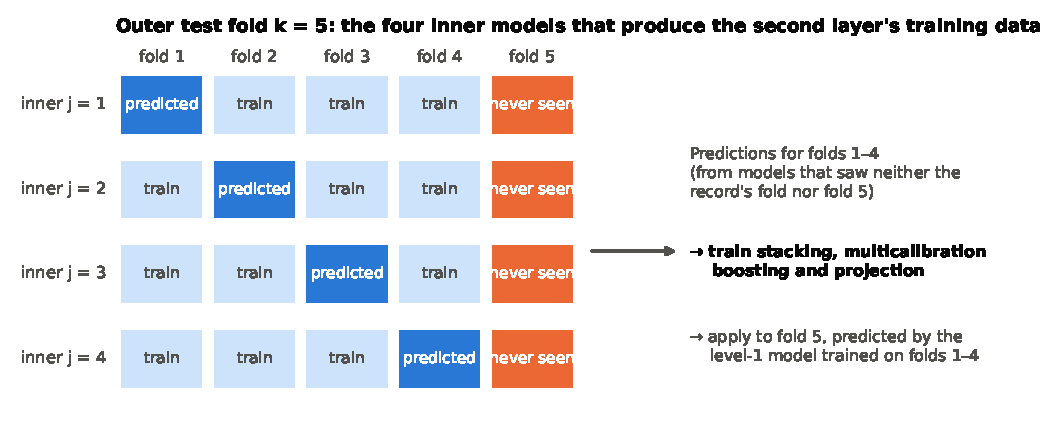
\includegraphics[width=\linewidth,height=145mm,keepaspectratio]{figures/x02_nested_scheme.pdf}
\captionof{figure}{Nested cross-fitting to generate second-layer training data for one outer test fold.}\label{fig:nested}
\end{center}
Nested fitting supplies the second layer with base predictions for records not directly used to train those predictors (Figure S1). This resembles applying score correction to new records and reduces optimism from using fitted training probabilities. Configurations were compared on the same outer records, allowing Table S4 to assess changes after each calibration step. The design isolates direct fitting; historical-information availability remains governed by Section S1.4.

{\small Nested predictions isolate direct base-learner training records. Historical information boundaries are described in Section S1.4.\par}
\clearpage

\begin{center}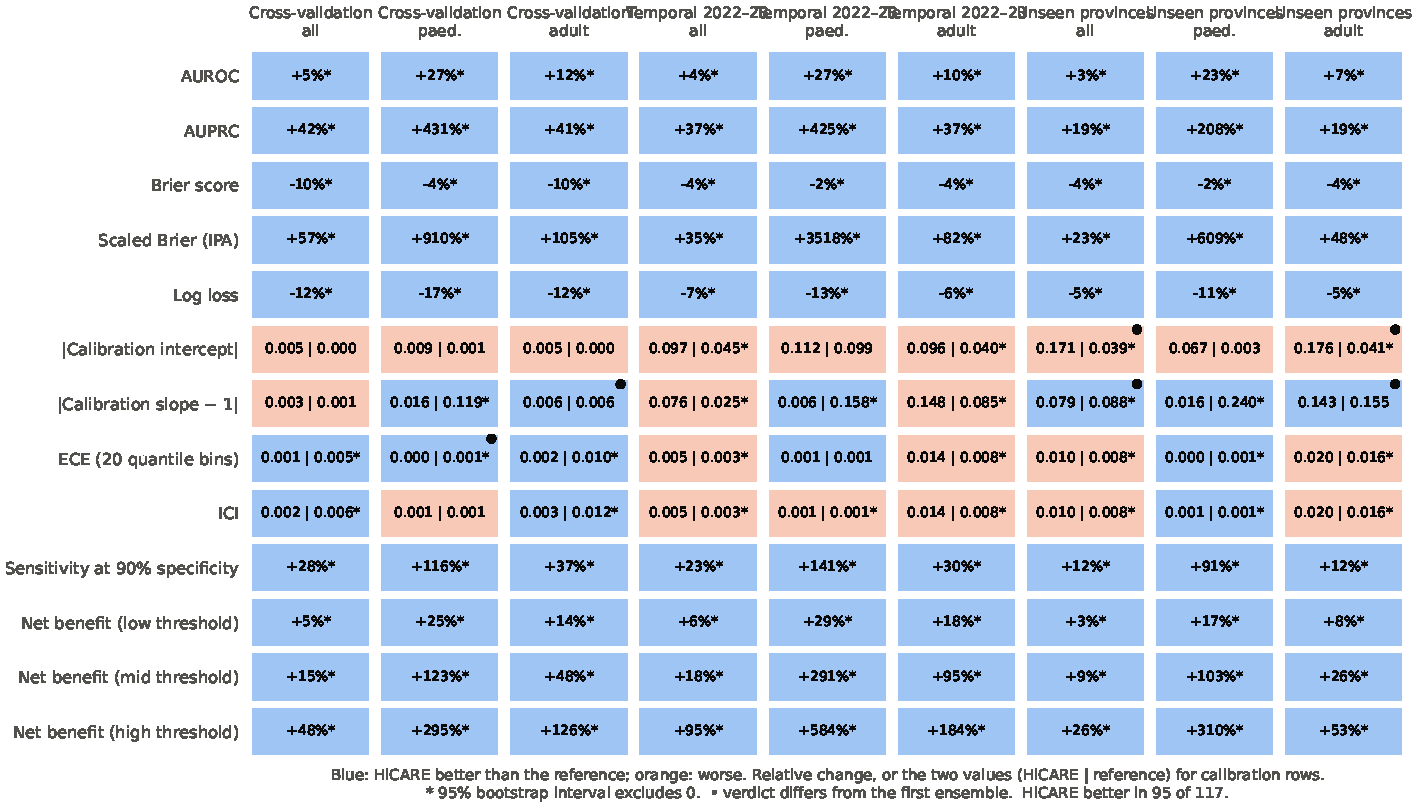
\includegraphics[width=\linewidth,height=145mm,keepaspectratio]{figures/x07_winloss.pdf}
\captionof{figure}{Comparisons across 13 metrics, three populations and three evaluation protocols.}\label{fig:winmap}
\end{center}
Figure S2 disaggregates performance by population and protocol. Advantages in ranking and related metrics were widespread, whereas calibration differences varied across tasks without a consistent direction. Relative risk relationships transferred more readily than absolute probability levels. Monthly updating and local intercept checks therefore address probability maintenance in different monitoring environments. These tasks support organising evaluation by error source rather than summarising performance with a single all-age metric.

{\small Geographic evaluation concerns the profile ensemble configuration. Colours denote differences from LR-7; stars and symbols denote statistical significance and changes relative to EW, as defined in the legend.\par}
\clearpage

\begin{center}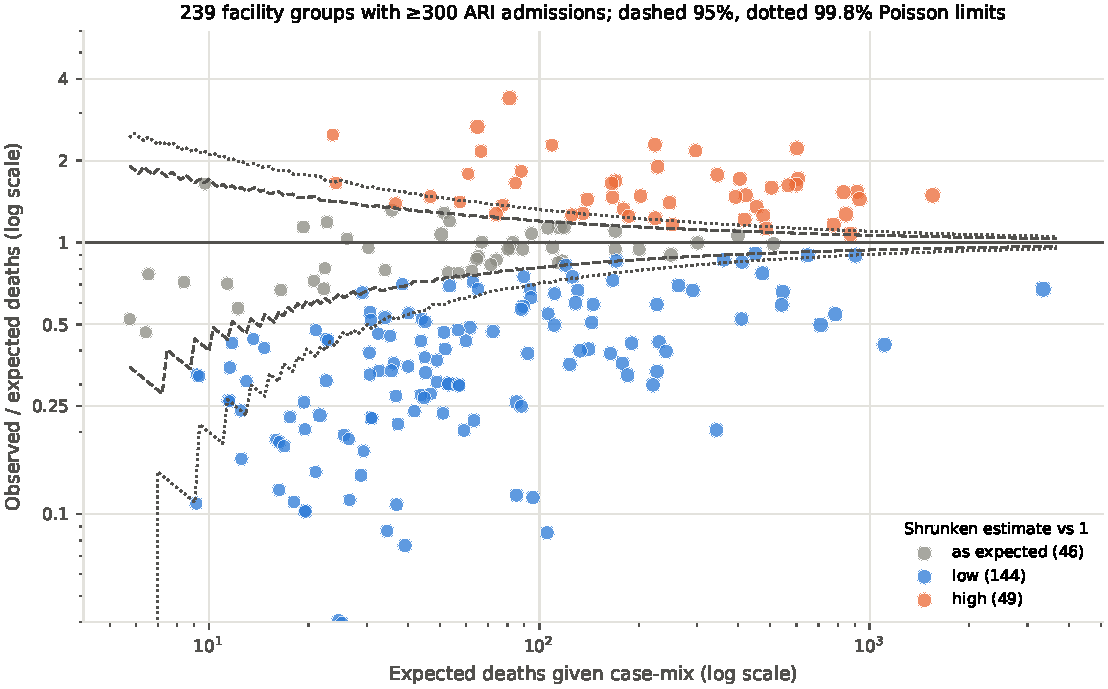
\includegraphics[width=\linewidth,height=145mm,keepaspectratio]{figures/m2_facility_funnel.pdf}
\captionof{figure}{Funnel plot of standardised mortality in facility groups.}\label{fig:funnel}
\end{center}
Among 239 eligible facility groups, 49 had shrinkage intervals above the reference, 144 below it and 46 without a clear departure (Figure S3). High-ratio groups accounted for approximately 8,629 more observed than expected deaths, locating national departures in a limited number of service units. The funnel plot also shows wider random variation at lower expected counts. Combining counts with shrinkage estimates helps prioritise large, well-supported departures. These units combine administrative and facility attributes and must still be linked to individual hospitals for investigation.

{\small Funnel control limits and empirical Bayes intervals have different statistical definitions. Facility groups combine administrative and institutional attributes and are not necessarily individual hospitals.\par}
\clearpage

\begin{center}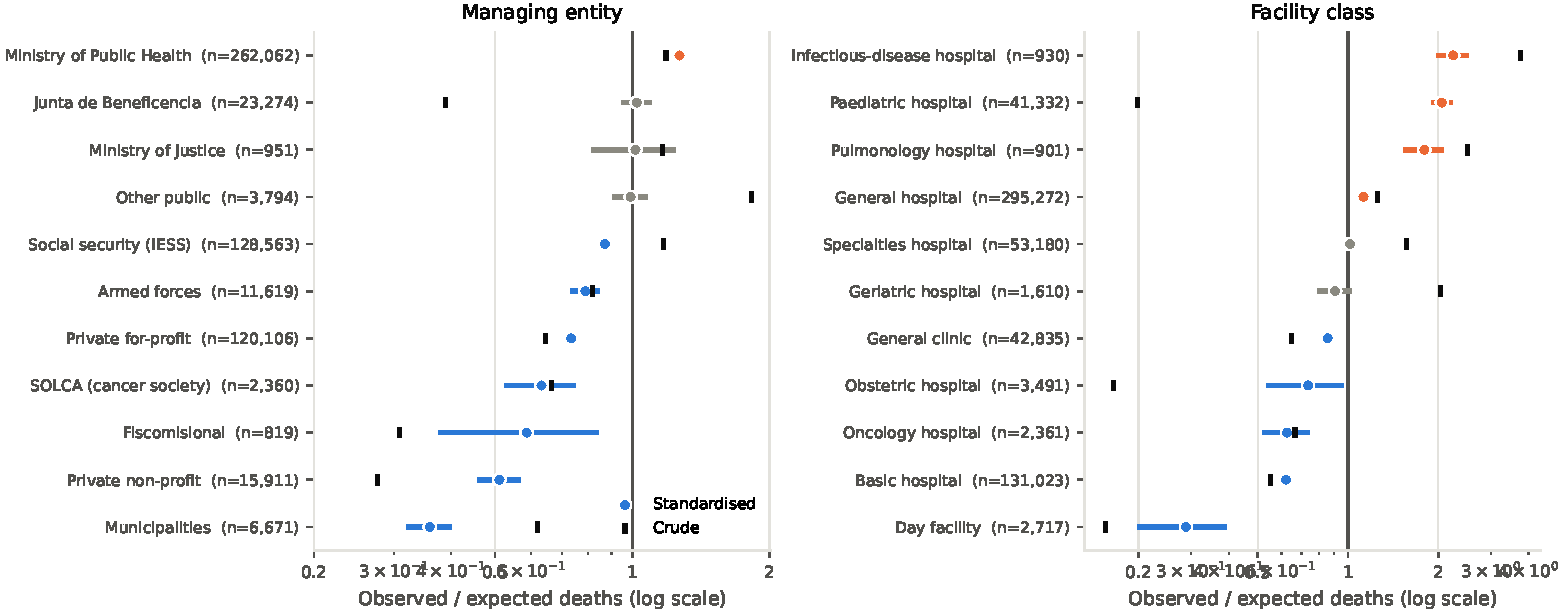
\includegraphics[width=\linewidth,height=145mm,keepaspectratio]{figures/m3_provider_type.pdf}
\captionof{figure}{Standardised mortality by administering entity and facility class.}\label{fig:entity}
\end{center}
The direction of movement from crude to standardised ratios differed by administering entity and facility class, most conspicuously for children’s hospitals (Figure S4). Case mix did not affect every facility type by a common multiplier, making national crude mortality an inadequate shared benchmark. This explains the two treatments of facility information. Prediction uses profiles to supplement patient records, whereas comparison first creates a common patient case-mix reference and examines the facility differences that remain. The former enriches risk description; the latter locates outcome departures requiring explanation.

\clearpage

\begin{center}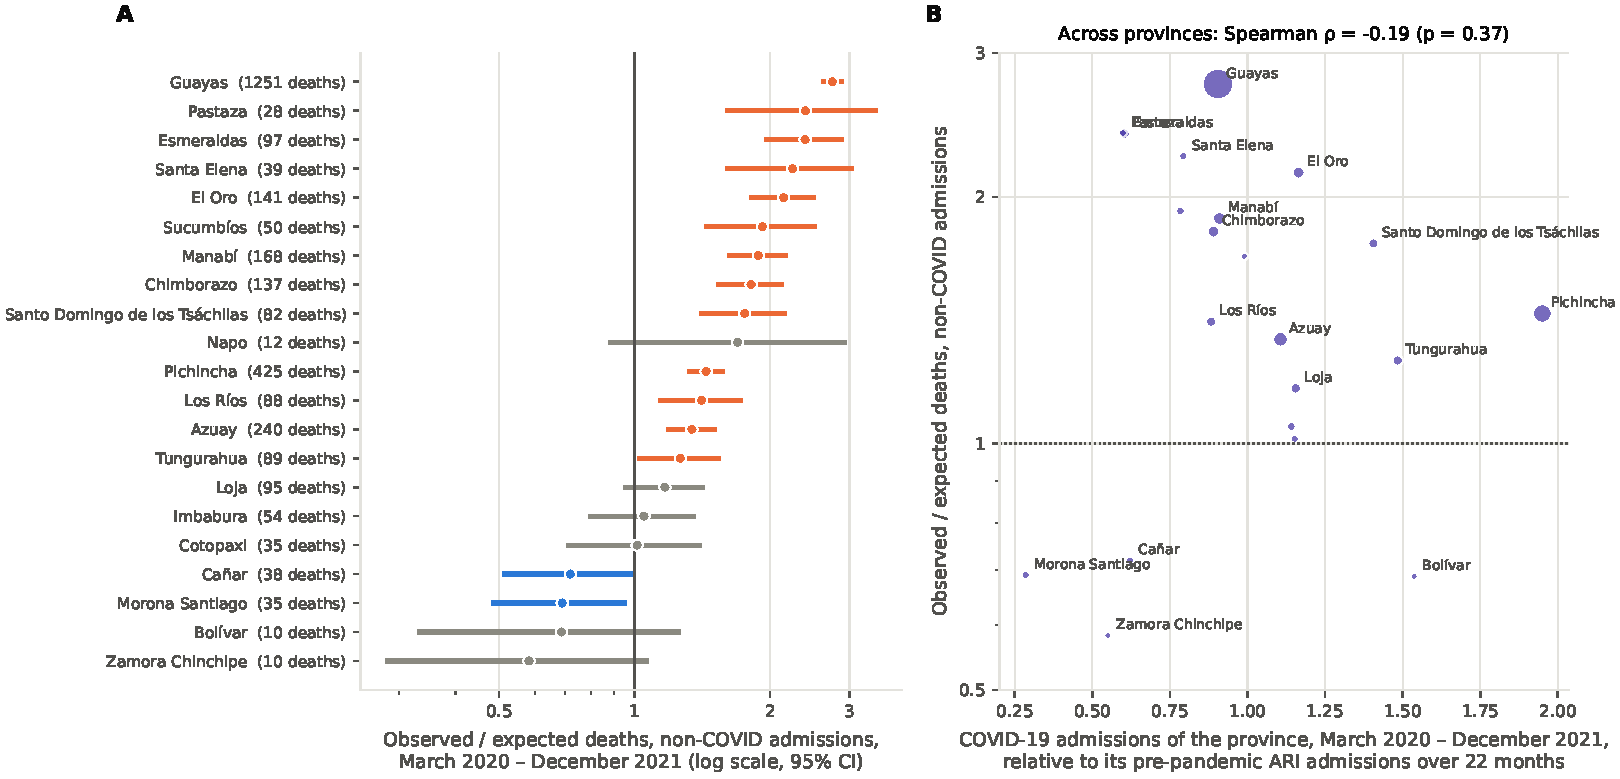
\includegraphics[width=\linewidth,height=145mm,keepaspectratio]{figures/x15_strain_by_province.pdf}
\captionof{figure}{Provincial non-COVID mortality departures from the historical reference during the pandemic. (A) Ratios and 95\% intervals. (B) Association with cumulative provincial COVID-19 demand.}\label{fig:strainprov}
\end{center}
At provincial scale, cumulative COVID-19 demand was not positively associated with non-COVID mortality ratios (r = $-$0.19, p = 0.37; Figure S5), unlike the facility-month pattern in Table S11. Co-occurrence of high contemporaneous facility demand and mortality departures therefore does not imply higher non-COVID ratios in provinces with more cumulative COVID-19 admissions. Provincial totals combine facilities, epidemic peaks and admission selection and describe a different quantity from monthly care processes. Interpretation should remain at the corresponding scale, with provincial mortality differences investigated using local service and registry information.

\clearpage

\begin{center}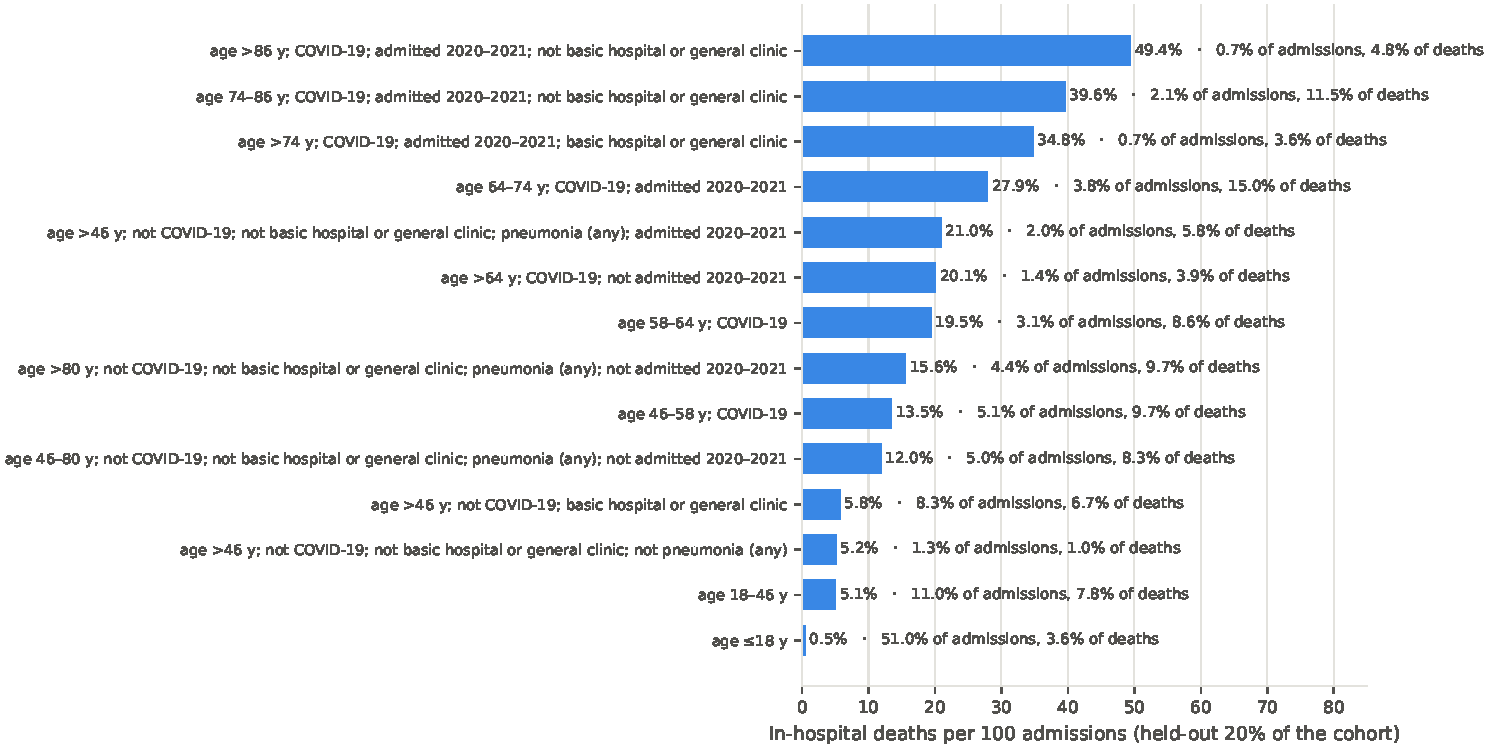
\includegraphics[width=\linewidth,height=145mm,keepaspectratio]{figures/m8_phenotypes.pdf}
\captionof{figure}{Deaths per 100 admissions in 14 risk-tree leaves evaluated on held-out data.}\label{fig:pheno}
\end{center}
Mortality differences between phenotypes demonstrate the discrimination of shallow rules (Figure S6). The age $\leq$18 leaf accounted for approximately 51.0\% of admissions and 3.6\% of deaths, with mortality of 0.5\%. The leaf for patients older than 86 with early-pandemic COVID-19 in specified facility classes had mortality of 49.4\%. These rules translate complex risk relationships into inspectable patient combinations, supporting stratified review. Because risk still varies within each phenotype, rules primarily aid interpretation, while continuous scores provide finer priorities.

\clearpage
\mainheading{S4 Extended interpretation of main-text figures}
The following sections retain stratified interpretations, comparison conditions and additional numerical details in main-text figure order. The main text integrates these findings into a continuous argument; this section clarifies the scope of each analysis.

\subheading{Figure 1. Risk estimation and independent population monitoring.}
Figure 1 traces the shared registry inputs into prediction and independent monitoring. Panel A links 33 base features and 18 facility-profile variables to model fitting, stratified calibration and monthly maintenance. Its cross-validation and temporal results connect these stages to discrimination and calibration, including the comparison with identically updated EW. Panel B instead defines separate expected values for each monitoring question. Case-mix adjustment supports regional comparisons, the fixed pre-pandemic risk relationship supports non-COVID period comparisons, and seasonal counts provide the paediatric demand reference. Provincial mortality ratios and the paediatric prediction interval therefore describe departures from these specific references rather than predictive gains attributable to HiCARE.

{\small Facility profiles comprise seven service statistics and eleven diagnostic-composition variables. Population standardisation uses independent models.\par}
\subheading{Figure 2. Facility profiles. (A) Mean non-ARI profiles by facility class. (B) Facility-group non-ARI all-cause mortality versus ARI mortality.}
Non-ARI age composition, length of stay and diagnostic-chapter proportions differed by facility class, indicating distinct service responsibilities (Figure 2A). The relationship between non-ARI all-cause mortality and ARI mortality connected these service differences to the target outcome (Figure 2B). Facilities serving complex cases or receiving cross-region referrals may retain similar characteristics across disease groups. Non-ARI profiles thus supplement ARI records with limited clinical fields. Their predictive role is examined further through attribution and province-held-out evaluation.

\subheading{Figure 3. HiCARE stratified calibration, temporal updating and evaluation protocols.}
Figure 3 expands the prediction branch into five panels. Panel A specifies base learners and their inputs; panel B links stratified stacking, residual correction and marginal projection to equations (2)–(4). The expanded stacking expression is equivalent to main-text equation (2) and equation (S2). Panel C confines monthly state updating to temporal maintenance. Panel D distinguishes nested cross-validation from temporal and province-grouped holdout, while panel E defines comparators and metric families. The province protocol evaluates profile ensembles without the full second layer. Hyperparameters are detailed in S1.4, state updating in S1.5, and metric conditions in S1.9. Precomputed history and shared outcomes between residual early stopping and projection remain relevant to interpreting these protocols.

\subheading{Figure 4. Cross-validated (A) receiver operating characteristic and (B) precision–recall curves.}
HiCARE and EW were close across most thresholds, while both remained separated from LR-7 within age strata (Figure 4). Consistent with Table S3, expanded models provided a stable ranking advantage for high-risk records. In children, this was especially evident in precision–recall curves. With paediatric mortality of only 0.53\%, AUPRC nevertheless remained low. The improvement concerns preferentially identifying deaths among many survivors; the required review volume still depends on the target recall.

\subheading{Figure 5. Cross-validated calibration in 20 predicted-risk quantile bins on logarithmic axes.}
Age-specific curves show how ranking gains translated to probabilities (Figure 5). HiCARE ICI was 0.0006 in children and 0.0033 in adults, with predictions generally close to observed frequencies across both risk ranges. Lower paediatric absolute error partly reflects lower baseline mortality, requiring examination of low-probability departures on logarithmic axes. Adult curves cover a broader range and describe probability agreement at moderate and high risk. Stratification makes both error patterns visible before group-level expected totals are assessed.

{\small The 20 bins are for visualisation. Tabulated ICI uses a 200-bin isotonic approximation; the two are not the same numerical estimator.\par}
\subheading{Figure 6. Cross-validated decision curves.}
Across the thresholds in Figure 6, HiCARE and EW had broadly similar net benefit and generally exceeded LR-7. Under the displayed false-positive cost assumptions, improved ranking could therefore support more favourable screening. Their small difference also agrees with their similar ROC and precision–recall curves. Registry review can use workload and false-positive costs to identify candidate thresholds. Figure 26 further displays review proportions against mortality coverage.

\subheading{Figure 7. Contributions of facility profiles and second-layer components in cross-validation.}
Sequential correction revealed a trade-off between group totals and within-group probabilities (Figure 7). Marginal projection reduced maximum absolute log(O/E) from 0.166 to 0.076, while worst-group ECE increased from 0.0050 to 0.0059. Projection directly constrains average group residuals, primarily improving predicted death totals. Within the same group, underprediction and overprediction can still cancel, explaining lower total error alongside slightly greater within-group error.

LR-7 illustrates the same distinction. Its mean marginal error was only 0.0006, yet worst-group ECE was 0.0183, compared with 0.0059 for HiCARE. Accurate group means can coexist with weak within-group risk characterisation. HiCARE preserved stronger ranking while lowering errors in specified group totals, providing complementary probability support for individual stratification and population aggregation.

\subheading{Figure 8. Observed-to-expected mortality in 42 specified marginal subgroups in cross-validation.}
Disaggregating the mean error across 42 marginal groups shows which predicted totals changed (Figure 8). Relative to EW, HiCARE reduced O/E departures in the most affected groups. LR-7 also approached 1 in some categories, consistent with their inclusion as model predictors. Together with Figure 7, this distinguishes accurate marginal means from sufficient within-group discrimination. For monitoring based on summed probabilities, Figure 8 evaluates the former; risk curves and within-group ECE assess complementary properties.

{\small The 42 groups are defined by age, sex, ethnicity, urban or rural residence, sector, infection type and year. They are neither disjoint populations nor all possible intersections.\par}
\subheading{Figure 9. Paired bootstrap differences between HiCARE and the reference model in cross-validation.}
Paired bootstrap results retained the direction of HiCARE’s ranking advantage over LR-7 under record resampling (Figure 9). AUROC and AUPRC difference intervals were above zero for all ages, children and adults, and log-loss intervals were below zero. Improvements therefore included discrimination and probability loss. AUROC gains were approximately 0.185 in children and 0.088 in adults, consistent with Table S3.

Calibration followed a different pattern. All-age and adult ICI decreased, while the paediatric difference was close to zero because LR-7 already had small absolute calibration error in low-risk children. Large ranking gains with limited ICI change indicate better differentiation of risk within children without a comparable change in average probability error. As in Table S4, risk identification and group calibration require separate interpretation.

\subheading{Figure 10. TreeSHAP attribution. (A) Leading features. (B) Attribution shares by feature group. (C) Historical facility non-ARI mortality and attribution.}
Facility profiles accounted for approximately 12\% of total SHAP attribution, with non-ARI all-cause mortality among the leading features (Figure 10). The model therefore used historical information beyond demographics and ARI diagnoses. Alongside the service differences in Figure 2, attribution suggests that profiles may capture service level, referral reach and case complexity. Historical non-ARI mortality should consequently be understood as a proxy for risk context rather than a facility-quality score. Attribution describes information use by the fitted model; performance in new regions is assessed in Section 4.6.

{\small The combined profile group contains 18 service-statistic and diagnostic-composition features.\par}
\subheading{Figure 11. Bimonthly observed-to-expected mortality in 2022–2023 under static prediction, rolling windows and state-space recalibration.}
Bimonthly O/E curves showed persistent temporal departure with static models, while rolling and state updating brought most windows closer to 1 (Figure 11). This located the full-period gains in Table S5 in specific months, showing reduced accumulation of total-count error. COVID-19 subgroup changes did not fully match the all-age pattern, making a single common correction insufficient. Separate COVID-19 and child offsets allowed the monthly state model to respond to group-specific changes.

\subheading{Figure 12. State-space recalibration in 2018–2023 using annual forward prediction from models fitted on preceding years. (A–D) Coefficients and 95\% interval bands. (E) O/E. (F) Configuration selection in development years.}
In annual forward evaluation, the COVID-19 offset changed from approximately +0.49 in 2020 to $-$0.53 in 2022 and $-$0.60 in 2023 (Figure 12). The same base score required probability corrections in opposite directions. Static O/E changed from 3.09 to 1.01 after updating in 2020, and from 0.72 to 0.95 in 2022, respectively reducing early underprediction and later overprediction.

These reversals explain why a fixed intercept may not remain adequate and why monthly maintenance should retain population-specific offsets. State coefficients summarise changes in the risk mapping arising from admission selection, treatment, coding and unrecorded severity. They locate groups and periods requiring maintenance, but identifying clinical causes requires more detailed information.

{\small This figure uses annual forward fitting and monthly updating in 2018–2023. Table S5 instead uses fixed development in 2015–2021 and testing in 2022–2023.\par}
\subheading{Figure 13. Transfer to unseen provinces with and without facility profiles.}
After geographic identifiers were removed, the profile configuration increased province-held-out AUROC from 0.8654 to 0.8750 and reduced log loss from 0.1913 to 0.1876 (Figure 13). Historical service statistics were therefore associated with better risk identification in unseen provinces. This extends the information use shown in Figure 10 from the training distribution to geographic transfer.

Meanwhile, the calibration intercept shifted from $-$0.004 to +0.171, indicating overall risk underprediction with profiles. Service representations can carry relative risk information while still requiring local probability adjustment. Because ensemble membership also changed, differences reflect the entire configuration; support for facility representations must be interpreted within that comparison.

{\small The geographic HiCARE label denotes the profile ensemble without the full second layer. Local historical non-ARI information was available during evaluation.\par}
\subheading{Figure 14. Provincial (A) AUROC and (B) observed-to-expected mortality when each province is excluded from direct model training.}
The profile configuration exceeded LR-7 in AUROC in 23 of 24 provinces, showing that its ranking advantage was not confined to a few regions (Figure 14). Median provincial absolute log(O/E) decreased from 0.18 without profiles to 0.15 with profiles; LR-7 had a value of 0.23. Predicted total-count errors therefore improved in the typical province.

Improvement in the provincial median can coexist with the national intercept departure in Figure 13. The former describes the centre of the provincial error distribution; the latter depends jointly on admission volumes and case mix. The transfer result is therefore best characterised as widespread ranking improvement, with probabilities requiring checks both nationally and within each province.

{\small Provinces were excluded from direct fitting, but precomputed national historical context could include their past outcomes. This is not external validation wholly free of local label information.\par}
\subheading{Figure 15. Provincial case-mix-standardised in-hospital mortality ratios, with empirical Bayes estimates and 95\% intervals; vertical tick marks indicate crude ratios.}
Case-mix adjustment materially changed provincial ordering (Figure 15). Sucumbíos increased from a crude ratio of 1.06 to 1.47, and Esmeraldas from 1.01 to 1.26. Near-average crude mortality therefore concealed higher mortality relative to their case mix. El Oro decreased from 1.79 to 1.56, indicating that higher-risk admissions explained part, but not all, of its departure. Opposing adjustment directions show that a common crude reference can both exaggerate and conceal differences, changing investigative priorities after standardisation.

\subheading{Figure 16. Observed minus expected in-hospital deaths by province, 2015–2023.}
Provinces with the strongest relative departures did not necessarily involve the most death records (Figure 16). Sucumbíos had a ratio of 1.47 and a difference of approximately 156 deaths; Guayas had a ratio of 1.11 but a difference of approximately 770, nearly five times larger. High admission volumes can make modest relative departures consequential in absolute numbers. Differences of approximately 1,276 in El Oro and 705 in Manabí combined relative departure with large scale. Reporting O/E beside O$-$E accommodates both. The approximately 3,932 deaths above expectation across high-ratio provinces are differences from a model reference, not avoidable deaths.

\subheading{Figure 17. Standardised mortality ratios by province, period and age stratum.}
Period stratification separated persistent from temporary departures (Figure 17). El Oro had ratios of 1.20, 1.68 and 1.51 across the three periods, remaining high after the pandemic. Esmeraldas increased from 0.89 to 1.49 before returning to 1.01. The former suggests examination of persistent case and service characteristics, while the latter concentrates attention on 2020–2021. El Oro also had an adult ratio of 1.59 versus 0.85 in children. Combined with Figures 15 and 16, these strata locate regional signals in particular periods and populations, improving the specificity of subsequent record review.

\subheading{Figure 18. Quarterly non-COVID ARI mortality O/E (left) and facility COVID-19 demand strata (right), with March 2020–December 2021 shaded.}
Quarterly curves located non-COVID mortality departures in the pandemic, while demand strata showed higher O/E in high-demand facility-months (Figure 18). The first identifies when departures occurred; the second narrows which service units require examination during that period. Together with the plateau among high-demand groups in Table S11, the findings suggest context-specific changes rather than a common linear demand effect across units. Subsequent investigations should preserve the facility-month scale.

\subheading{Figure 19. Monthly (A) COVID-19 admissions, (B) non-COVID ARI admissions and (C) observed-to-expected mortality among non-COVID admissions.}
Non-COVID admissions fell during the pandemic while O/E rose (Figure 19). Admission volume and mortality among admitted patients therefore describe different quantities. Changes in admission thresholds, attendance by mild cases and referral composition can concentrate risk in fewer registered patients. Residual departures after case-mix adjustment require investigation of factors incompletely captured in the records. Tracking admissions alongside standardised mortality avoids equating lower admission volume with lower demand or outcome burden.

\subheading{Figure 20. Sequentially adjusted relative mortality ratios (left) and deaths within 48 hours as a proportion of deaths (right).}
Death timing provided an additional clue to paediatric differences (Figure 20). Among children who died, approximately 45\% of Indigenous children died within 48 hours compared with 21\% of Mestizo children; proportions were approximately 29\% for rural and 21\% for urban children. Higher adjusted mortality co-occurred with more concentrated early deaths, directing attention to severity at arrival, pre-hospital illness and referrals. Early-death proportions describe timing among deaths and cannot distinguish severity from delay, but can narrow the information needed for review.

{\small Sequential adjustment estimates relative mortality under different conditioning sets. In public–private comparisons, ratios approaching 1 after inclusion of sector-related variables do not establish a causal explanation.\par}
\subheading{Figure 21. Age-specific paediatric non-COVID ARI admissions relative to the pre-pandemic seasonal counterfactual.}
Recovery was concentrated at ages 1–9 (Figure 21). In 2023, admission ratios were 1.54 at ages 1–4 and 2.03 at ages 5–9, compared with 1.10 in infants and 1.06 at ages 10–19. The aggregate increase therefore did not imply proportional growth across ages, directing particular attention to preschool and younger school-age children. The cumulative paediatric ratio from March 2020 to 2023 was still 0.73, showing that high late-period admissions coexisted with fewer admissions across the entire period. Annual recovery and cumulative burden require separate interpretation.

{\small Expected infant and age 1–4 counts use the same population trend for ages 0–4. Intervals are predictive intervals around the seasonal benchmark.\par}
\subheading{Figure 22. Quarterly observed-to-expected non-COVID ARI admission ratios by age, 2019–2023.}
Quarterly decomposition showed age differences in the pace of recovery (Figure 22). All paediatric groups remained below seasonal baseline in early 2022, but age 1–4 and age 5–9 ratios reached 1.71 and 1.58 in the second quarter. Ages 5–9 remained high throughout 2023 and reached 2.29 in the second quarter, whereas infants were still at 0.73 in the first quarter. Sustained growth among older children thus coexisted with seasonal infant fluctuations. Annual totals obscure this concentration; quarterly or monthly information can support the evaluation of staffing and bed preparation.

\subheading{Figure 23. Syndrome-specific rebound and age shifts among admissions in children under 5.}
Syndrome strata connected age shifts to diagnostic categories (Figure 23). Pneumonia admissions at ages 1–4 in 2023 were approximately 1.64 times the fixed baseline, and the proportion aged at least 1 among under-5 pneumonia admissions increased from approximately 62\% to 72\%. Recovery was therefore concentrated beyond infancy, consistent with the age 1–4 increase in Figure 21. Separate series for pneumonia in older children and infant bronchiolitis are needed to describe recovery in these distinct populations.

{\small Age-specific expected counts are affected by approximate population denominators. Composition percentages describe observed admissions in the registry.\par}
\subheading{Figure 24. Monthly distributions of paediatric admissions before the pandemic and in 2022 and 2023.}
Syndromes also differed in peak timing (Figure 24). Before the pandemic, pneumonia at ages 1–9 was concentrated in January–February and infant bronchiolitis in February–March. Both peaks shifted to May–June in 2022. In 2023, the correlation with the pre-pandemic monthly distribution recovered to 0.83 for pneumonia but only 0.44 for bronchiolitis, indicating different degrees of seasonal recovery. Aggregating all paediatric respiratory admissions could conceal this timing difference. Alongside evidence of regional seasonality in Ecuador [20], these results support syndrome-specific local demand windows.

\subheading{Figure 25. Paediatric non-COVID ARI admissions in 2023 relative to provincial pre-pandemic seasonal incidence.}
Recovery also varied geographically (Figure 25). In 2023, ten provinces exceeded their own seasonal reference and two fell below it. Ratios were 2.47 in Bolívar, 1.95 in Pichincha, 1.90 in Zamora Chinchipe and 1.70 in Loja, compared with approximately 1.03 in Guayas. The national ratio of 1.32 therefore did not represent a common provincial change. Pichincha combined a high ratio with large admission volume, whereas Bolívar had stronger relative growth from a smaller baseline. As in regional mortality investigation, preparation should combine relative changes and local counts before linking them to length of stay and capacity.

\subheading{Figure 26. Mortality coverage against admission-review proportion when records are ranked by predicted risk.}
Continuous scores captured more deaths at the same review proportion. HiCARE and EW curves were close, generally above LR-7, and all-age curves exceeded ranking by 14 phenotypes (Figure 26). This translates discrimination into an interpretable review workload. Shallow phenotypes describe patient categories, whereas continuous scores refine priorities within categories. Age-specific curves confirm that gains do not arise solely from adult–child risk differences. Coverage measures retrospective screening ability. Practical evaluation should choose review proportions according to capacity and record the problems identified and subsequent outcomes.

\subheading{Figure 27. Observed deaths per 100 admissions by age, infection group and period, with 95\% interval bands.}
Age-risk curves varied by infection and period, explaining why fixed phenotype rules require maintenance (Figure 27). Adult non-COVID pneumonia mortality was high in 2020–2021, whereas COVID-19 mortality declined in 2022–2023. The same age therefore did not imply a common death probability across infections and periods. This agrees with the reversal in COVID-19 offsets in Figure 12 and provides population-level support for infection-specific probability maintenance. Age remained an important stratifier, but its probability scale required interpretation in the current infection mix and period.

\end{document}
